\chapter{Manual de Instalare și Utilizare}
\pagestyle{fancy}

\section{Instalare}
\subsection{Condiții prealabile generale}
\noindent Resursele hardware necesare pentru instalarea și rularea aplicației sunt:
\begin{itemize}
    \setlength\itemsep{0.5em}
    \item Sistem de operare: Windows
    \item Arhitectura sistemului de operare: x64
    \item Memorie RAM: minim 8GB
\end{itemize}

\subsection{Condiții prealabile pentru baza de date}
Este de preferat să fie instalate versiunile cele mai noi, {\it Long Term Support}.\\

\noindent Pentru instalarea resurselor necesare bazei de date, este nevoie de:
\begin{itemize}
    \setlength\itemsep{0.5em}
    \item \href{https://www.microsoft.com/en-us/sql-server/sql-server-downloads}{\color{blue}SQL Server}
    \begin{itemize}
        \setlength\itemsep{0.5em}
        \item Se descarcă din secțiunea Free Specialized Edition -> Developer
        \item Se deschide fișierul descărcat și se urmează instrucțiunile până la tipul instalării. Aici se va selecta {\it Basic}
        \item După ce instalarea a fost finalizată cu succes, se apasă butonul de {\it Install SSMS} 
        \item După ce SSMS a fost instalat, deschideți Microsoft SQL Server Management Studio
        \item Pentru Server Type se poate păstra Database Engine, iar pentru Authentication se va selecta Windows Authentication
    \end{itemize}

    \item \href{https://docs.microsoft.com/en-us/sql/ssms/download-sql-server-management-studio-ssms?view=sql-server-ver16}{\color{blue}SQL Server Management Studio (SSMS)}
    \begin{itemize}
        \setlength\itemsep{0.5em}
        \item Se deschide fișierul descărcat, se va selecta locația unde se dorește a fi instalat, apoi se apasă pe butonul de Install
        \item După ce instalarea e completa, e nevoie să fie restartat calculatorul 
    \end{itemize}
\end{itemize}

După ce toate instalările au fost finalizate cu succes, se pot crea baze de date, tabele și se pot efectua diferite comenzi și interogări.
\subsection{Condiții prealabile pentru modulul de backend}
Aplicația a fost creată utilizând .NET 6. De preferat, a se folosi această versiune, pentru că este posibil să fie modificări în versiunile ulterioare sau anterioare ce implică o sintaxă diferită.
Spre exemplu, la trecerea de la .NET 5 la .NET 6, fișierele Program.cs și Startup.cs au fost comasate.
\begin{itemize}
    \setlength\itemsep{0.5em}
    \item \href{https://dotnet.microsoft.com/en-us/download}{\color{blue}.NET 6}
    \begin{itemize}
        \setlength\itemsep{0.5em}
        \item Se apasă butonul Download {\it .NET SDK x64}, versiunea .NET 6.0, LTS
        \item Din pagina unde s-a făcut redirecționarea după apăsarea pe buton, se va selecta Installer-ul potrivit pentru sistemul de operare
        \item După descărcare, se va deschide fișierul executabil și se vor urma instrucțiunile
        \item Se poate testa într-un command line dacă instalarea s-a făcut cu succes, scriind {\it dotnet --info}
    \end{itemize}
    \item IDE: \href{https://www.jetbrains.com/rider/download/#section=windows}{\color{blue}Rider}
    \begin{itemize}
        \setlength\itemsep{0.5em}
        \item Se poate descărca de pe site-ul oficial sau din \href{https://www.jetbrains.com/toolbox-app/}{\color{blue}Jetbrains Toolbox}
        \item Se acceptă toate setările default
    \end{itemize}
\end{itemize}

\subsection{Condiții prealabile pentru modulul de frontend}
\begin{itemize}
    \setlength\itemsep{0.5em}
    \item Node v16.13.0
    \begin{itemize}
        \setlength\itemsep{0.5em}
        \item Se poate descărca \href{https://nodejs.org/en/download/}{\color{blue}de aici}
        \item Se acceptă toate setările default
    \end{itemize}
    \item Node Package Manager (npm) 8.1.0
    \begin{itemize}
        \setlength\itemsep{0.5em}
        \item Se poate descărca \href{https://nodejs.org/en/download/}{\color{blue}de aici}
        \item Se acceptă toate setările default
    \end{itemize}
    \item Text Editor: Visual Studio Code
    \begin{itemize}
        \setlength\itemsep{0.5em}
        \item Se poate descărca \href{https://code.visualstudio.com/download}{\color{blue}de aici}
        \item Se acceptă toate setările default
    \end{itemize}
\end{itemize}

\section{Rulare}
\subsection{Setup baza de date}
Dacă apar erori legate de baza de date, trebuie să se creeze una manual care să coincidă cu numele din fișierul appsettings.json din modulul de backend.
\subsection{Rulare modul backend}
La prima utilizare, trebuie să se importe proiectul și să se ruleze configurarea IIS Express. Se va rula comanda {\it dotnet ef database update} pentru a fi actualizată baza de date și pentru a fi create tabelele care vor fi ulterior folosite.
\begin{figure}[ht]
	\centering
	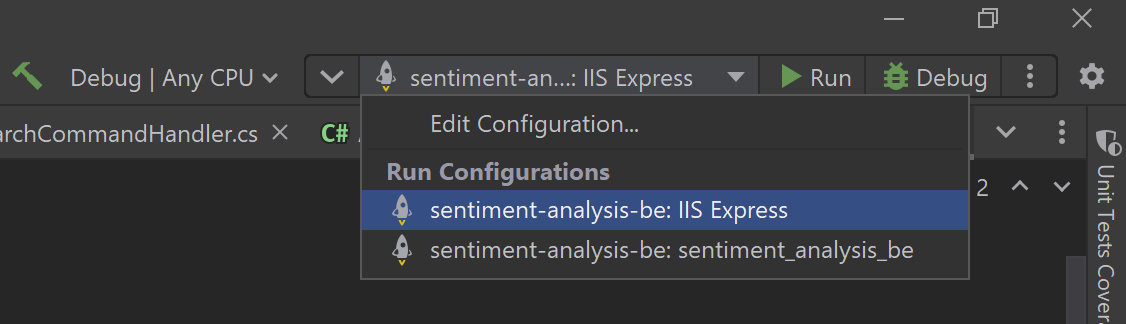
\includegraphics[width=150mm]{figs/configBackend.png}
    \caption{Configurări rulare backend}
	\label{fig:configBackend}
\end{figure}

Aplicația va deschide în broswer Swagger cu {\it https://localhost:44329/swagger/index.html}, un instrument care permite testarea și documentarea serviciilor REST.
\begin{figure}[H]
	\centering
	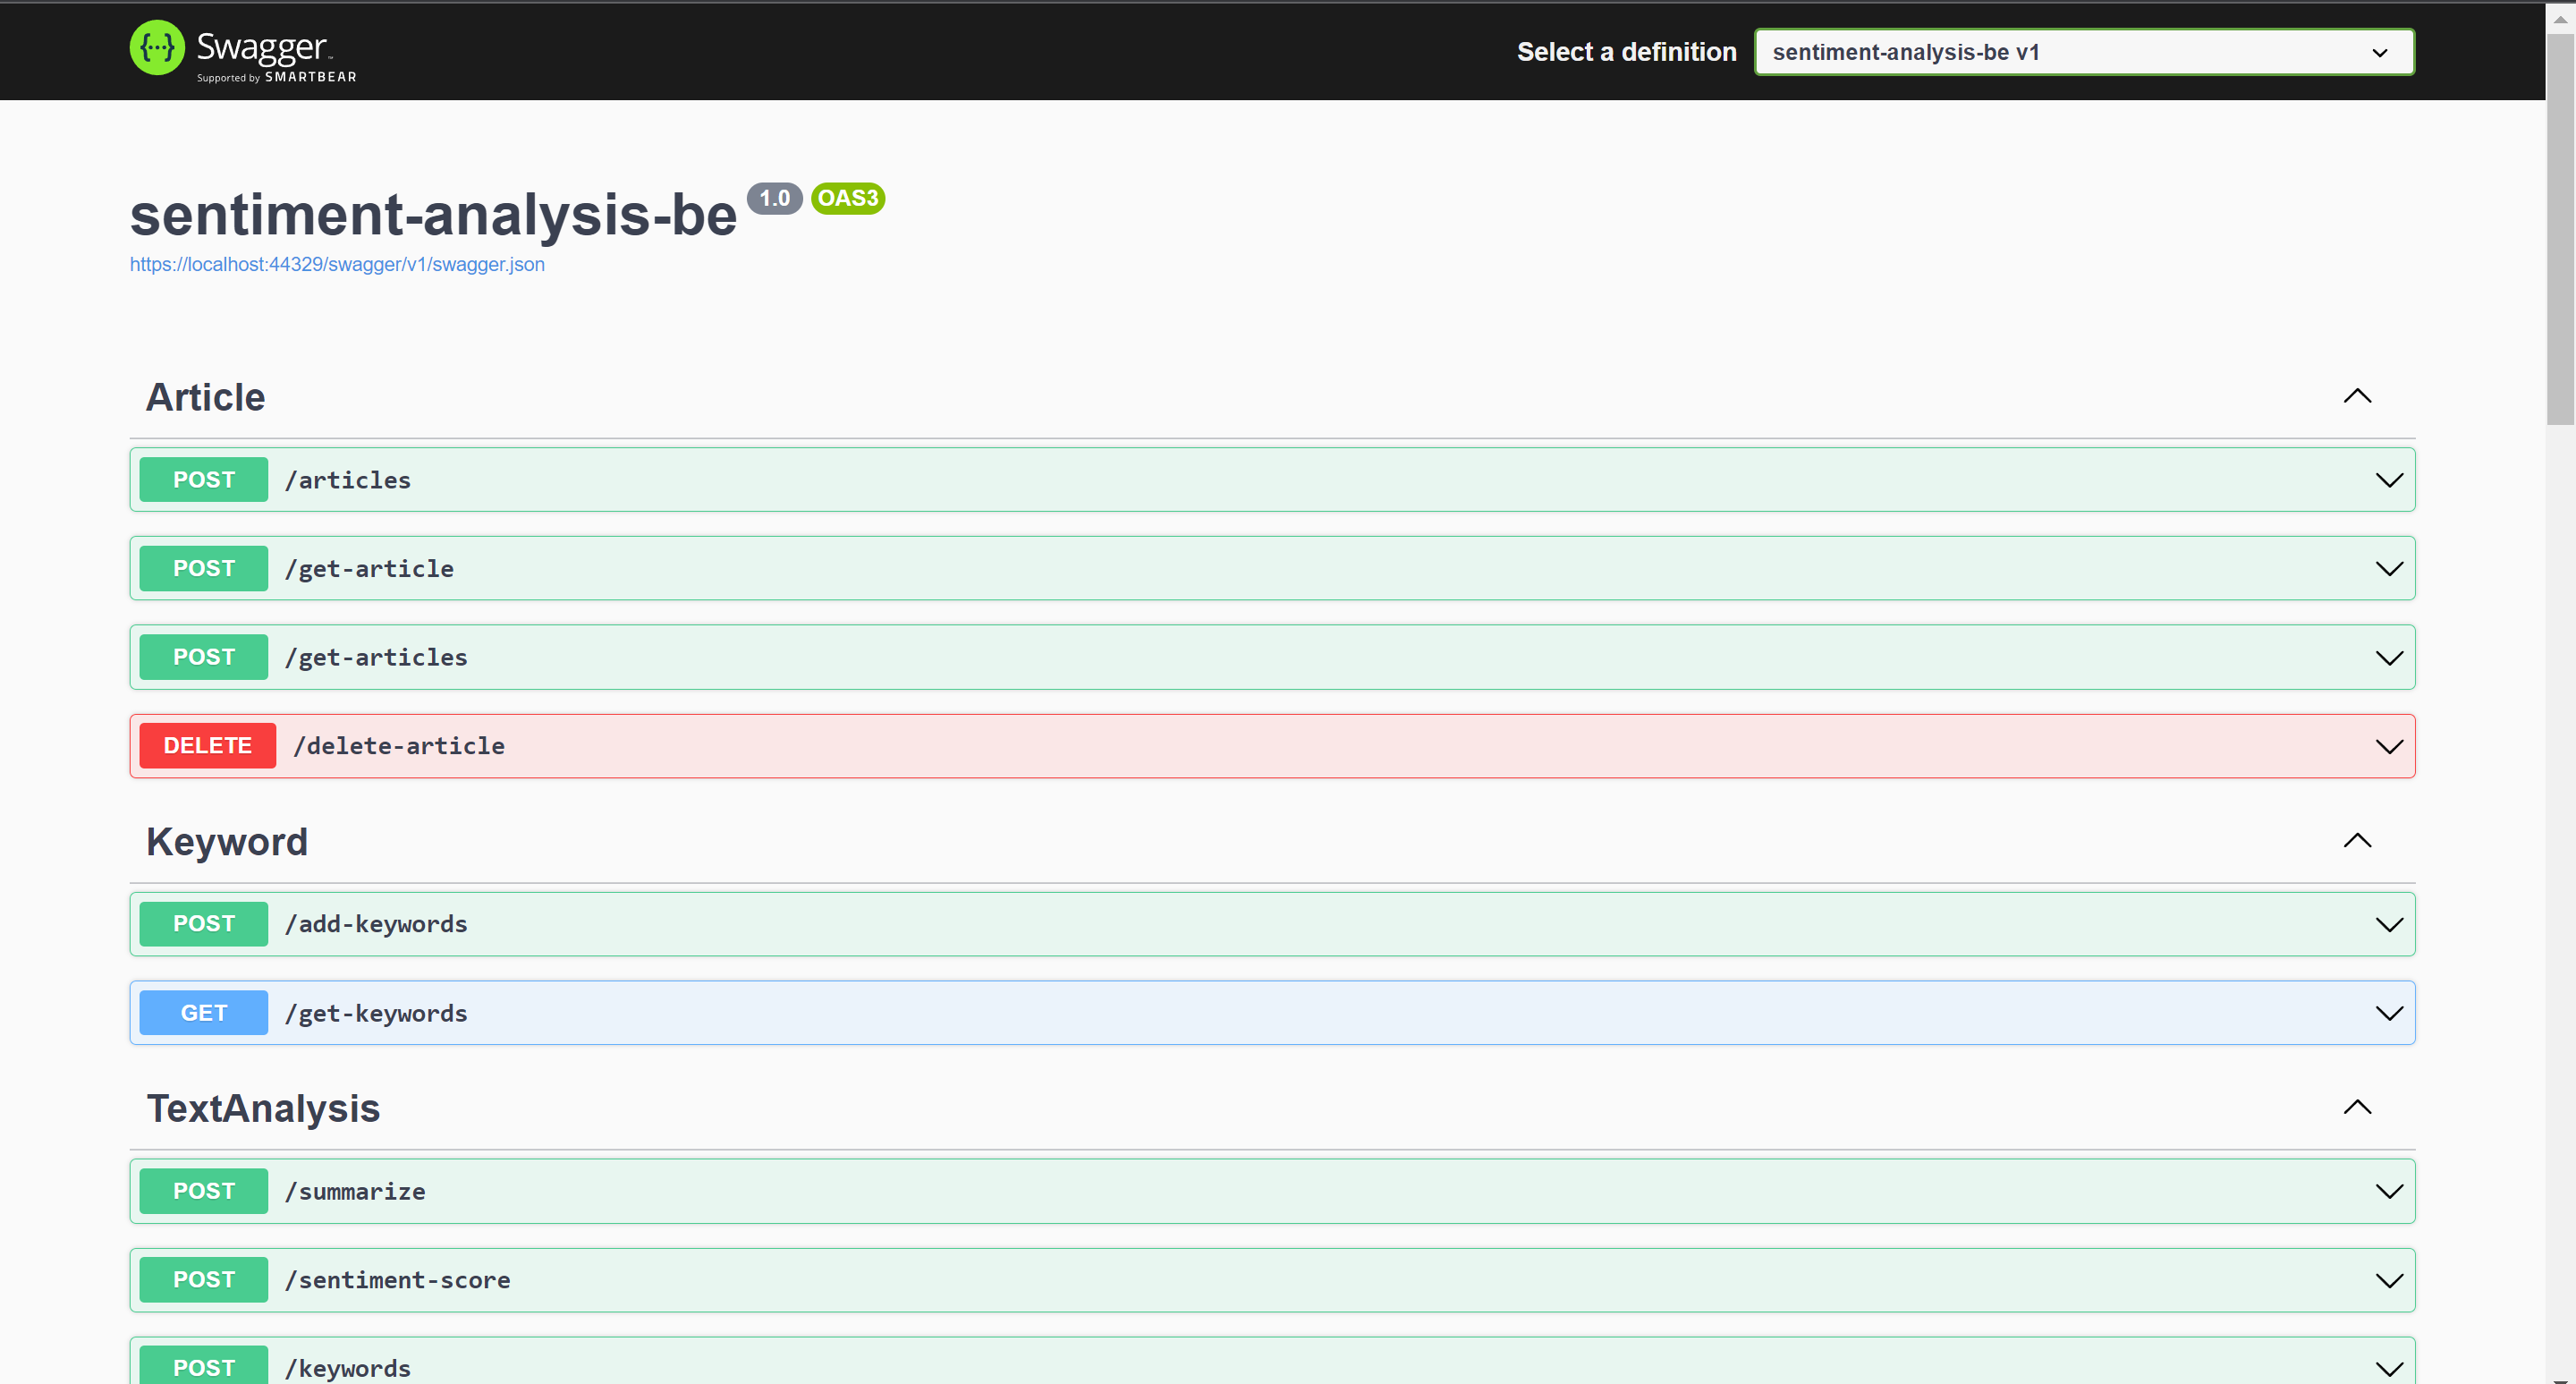
\includegraphics[width=150mm]{figs/swagger.png}
    \caption{Swagger, instrument pentru testarea endpointurilor aplicatiei}
	\label{fig:swagger}
\end{figure}
În acest moment, backend-ul rulează pe portul 44329 la care se va conecta modulul de frontend pentru a folosi API-ul creat.
\subsection{Rulare modul frontend}
După instalarea editorului de text Visual Studio Code, se va importa proiectul aici. Pentru a fi instalate toate dependințele necesare rulării proiectului, 
se va rula în terminal {\it npm init}. 
După ce toate dependințele au fost descărcate și instalate cu succes, se poate rula în terminal comanda {\it npm start}. După ce aplicația a pornit, se va deschide în broswer un tab de React App cu {\it http://localhost:3000/login}.
\begin{figure}[ht]
	\centering
	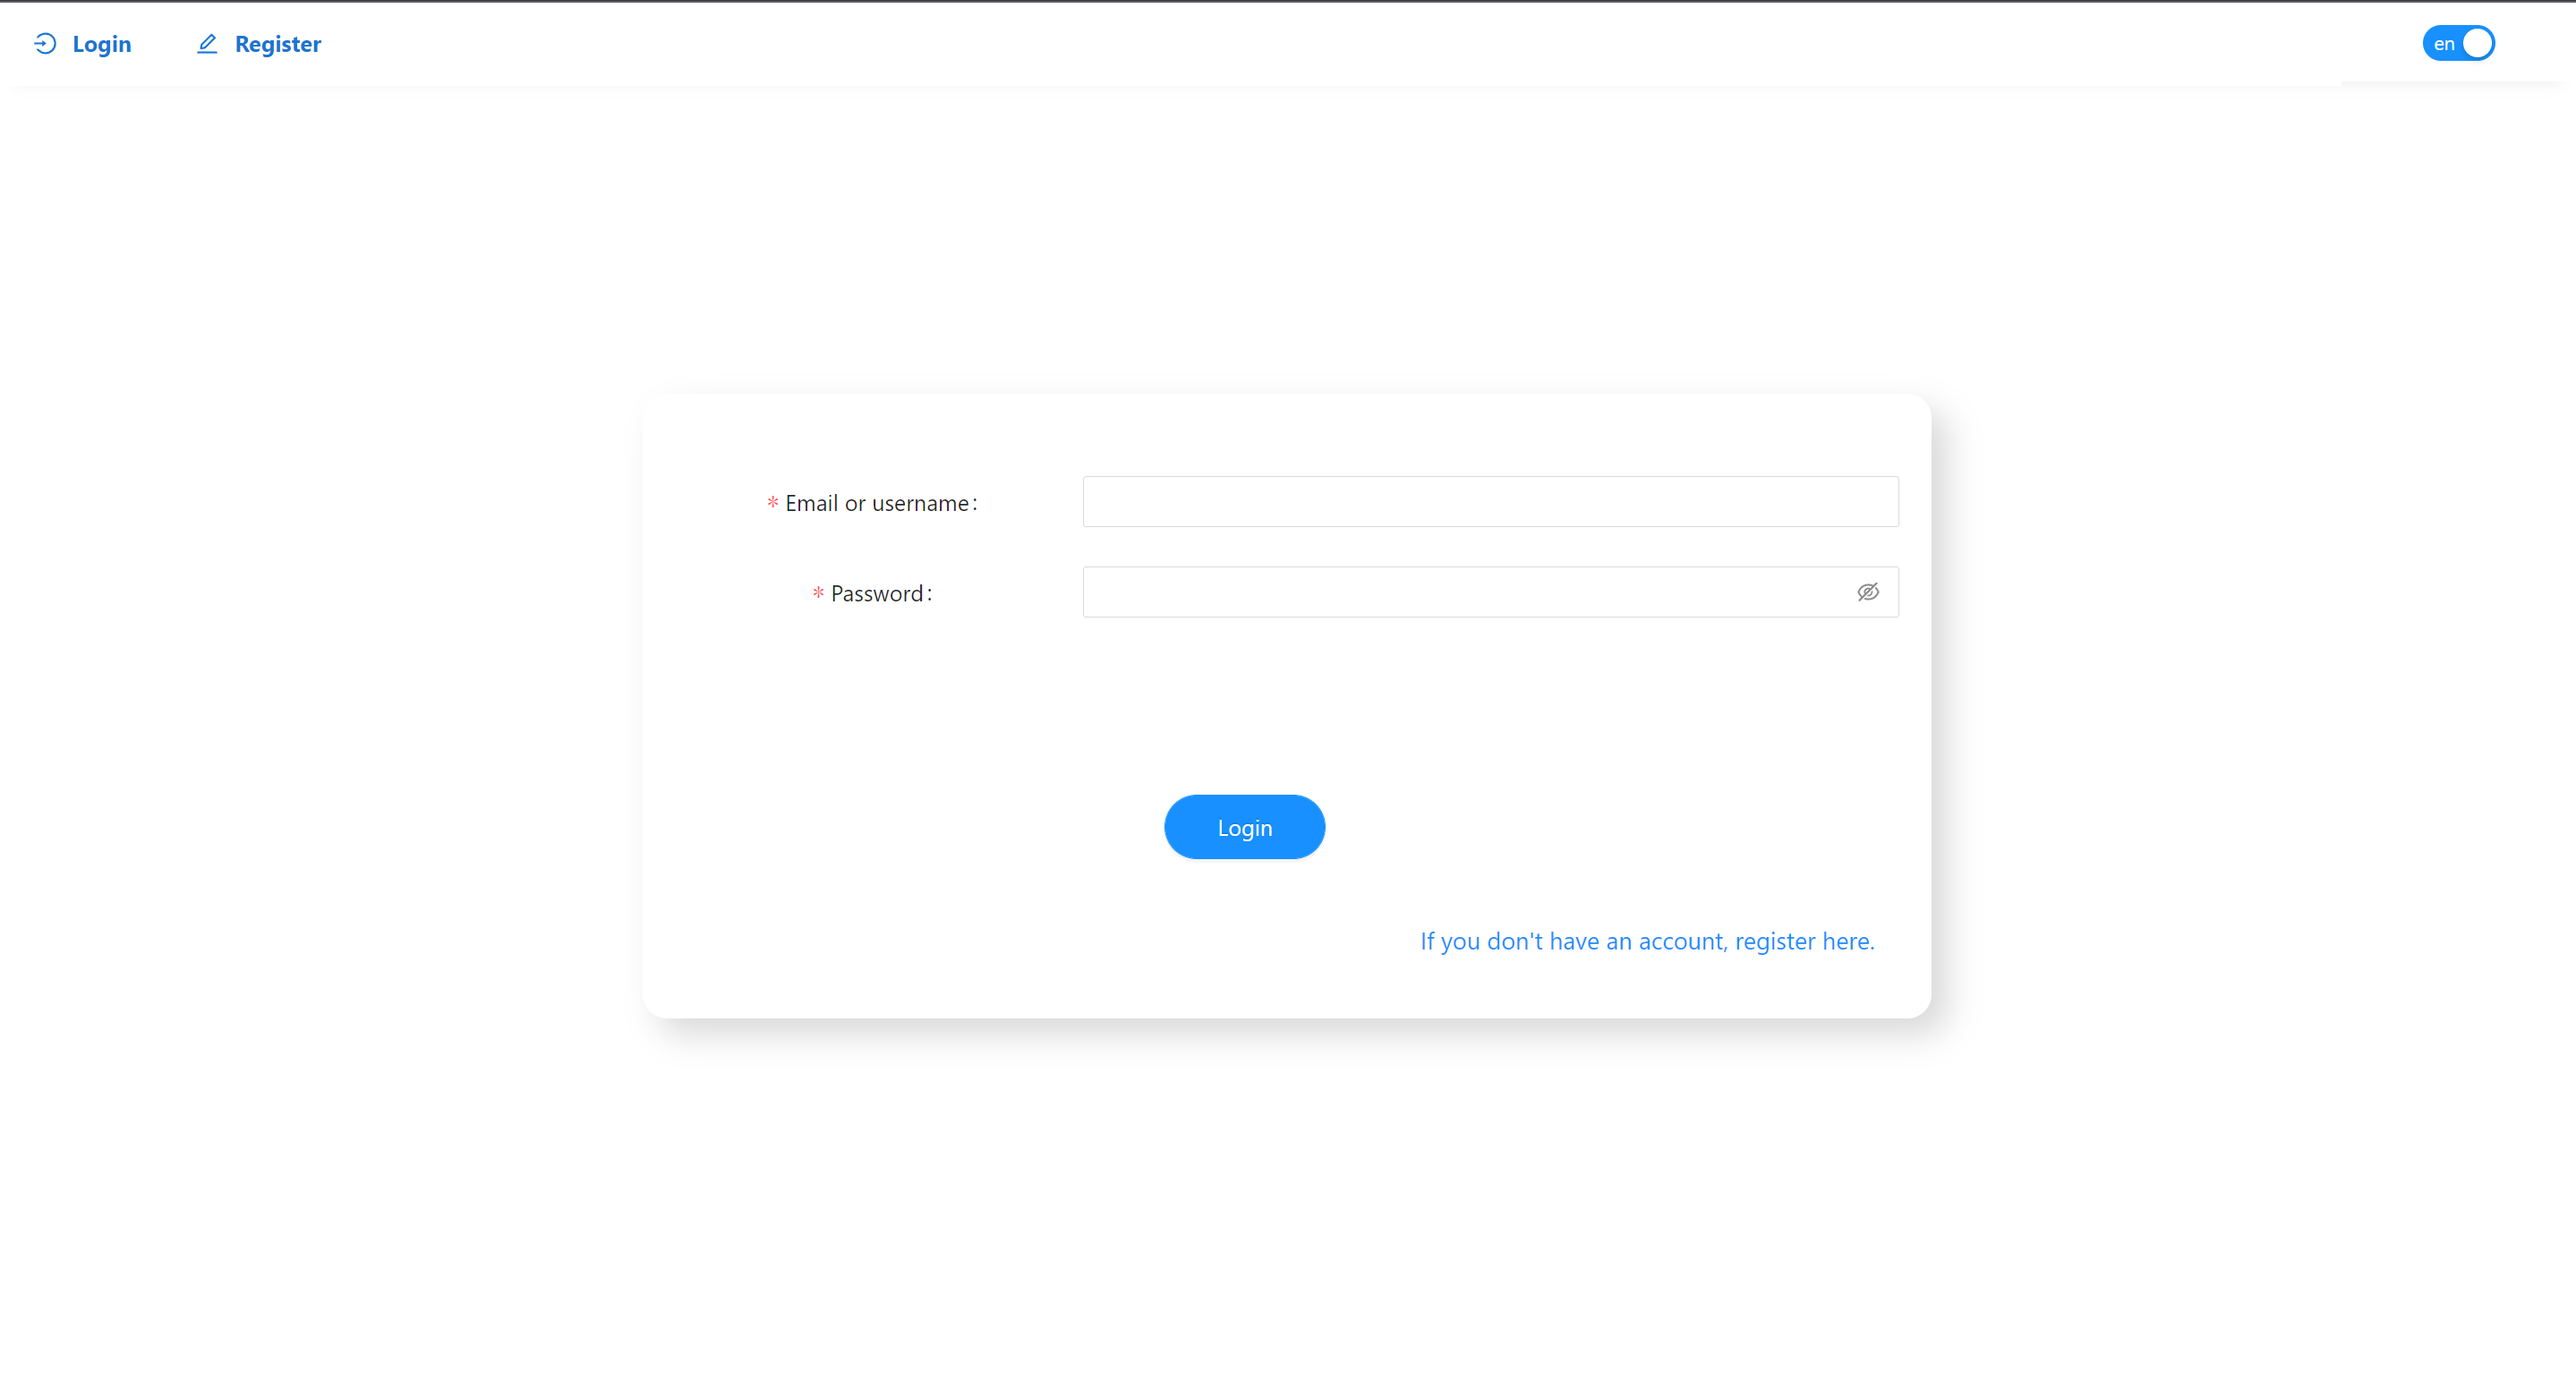
\includegraphics[width=150mm]{figs/startAppFrontend.png}
    \caption{Rulare frontend}
	\label{fig:startAppFrontend}
\end{figure}

\section{Manual de utilizare}
La pornirea aplicației, dacă nu a folost logat niciun alt utilizator înainte, prima pagină care se va deschide va fi pagina de login.
În funcție de preferințele utilizatorului, acesta poate modifica limba aplicației cu ajutorul switch-ului de limbi. Această setare poate fi modificată și mai târziu.

Pentru crearea unui cont nou, se va apăsa pe butonul indicat în figura \ref{fig:loginPage}. După ce am ajuns pe pagina de Register sau Creare cont nou, utilizatorul va trebui să completeze datele.
Aplicația ofera feedback vizual utilizatorului atunci când informațiile introduse de acesta în pagină nu respectă una dintre condițiile de număr minim, număr maxim de caractere format corect pentru email. Acest lucru se poate vedea în figura \ref{fig:createAccount}.
După ce toate câmpurile au fost corect completate din punct de vedere al restricțiilor menționate mai sus, se mai fac 2 verificări - numele de utilizator și email-ul să fie unice.
În cazul în care una din ele nu respectă condiția de unicitate, utilizatorul va fi notificat cu un mesaj corespunzător pentru a putea lua măsuri, după cum se poate vedea în figura.

\begin{figure}[ht]
	\centering
	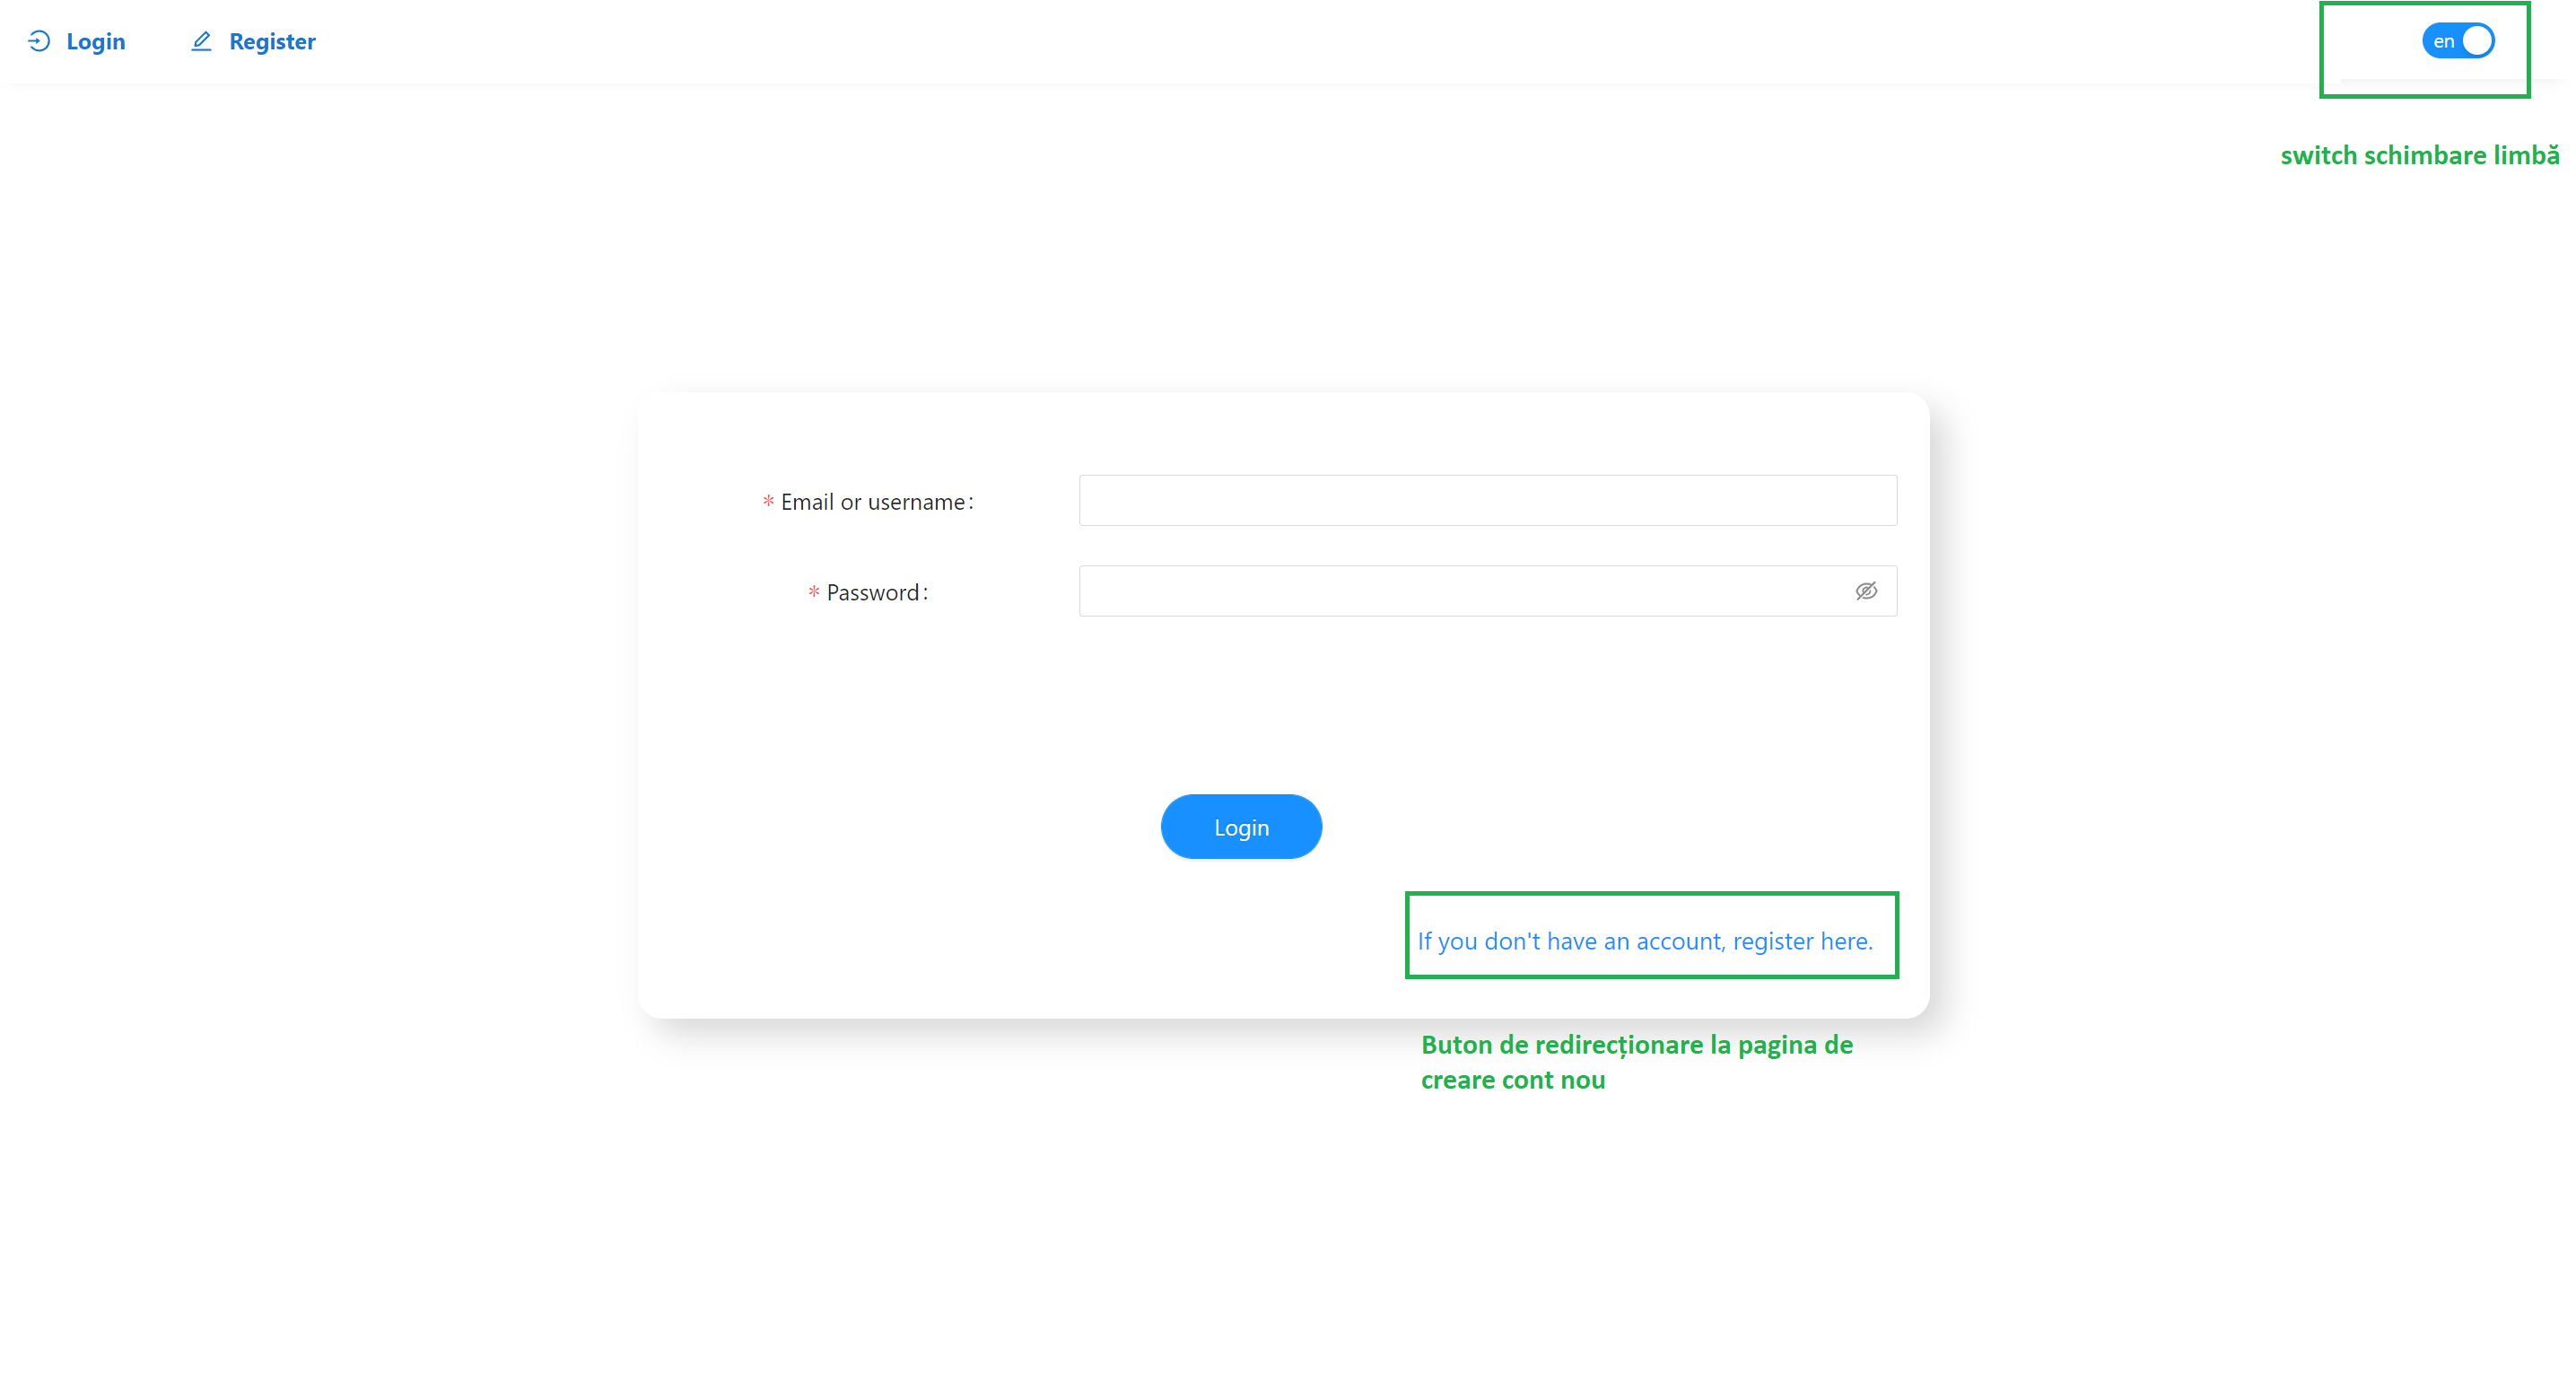
\includegraphics[width=100mm]{figs/loginPage.png}
    \caption{Pagina de login}
	\label{fig:loginPage}
\end{figure}

\begin{figure}[ht]
	\centering
	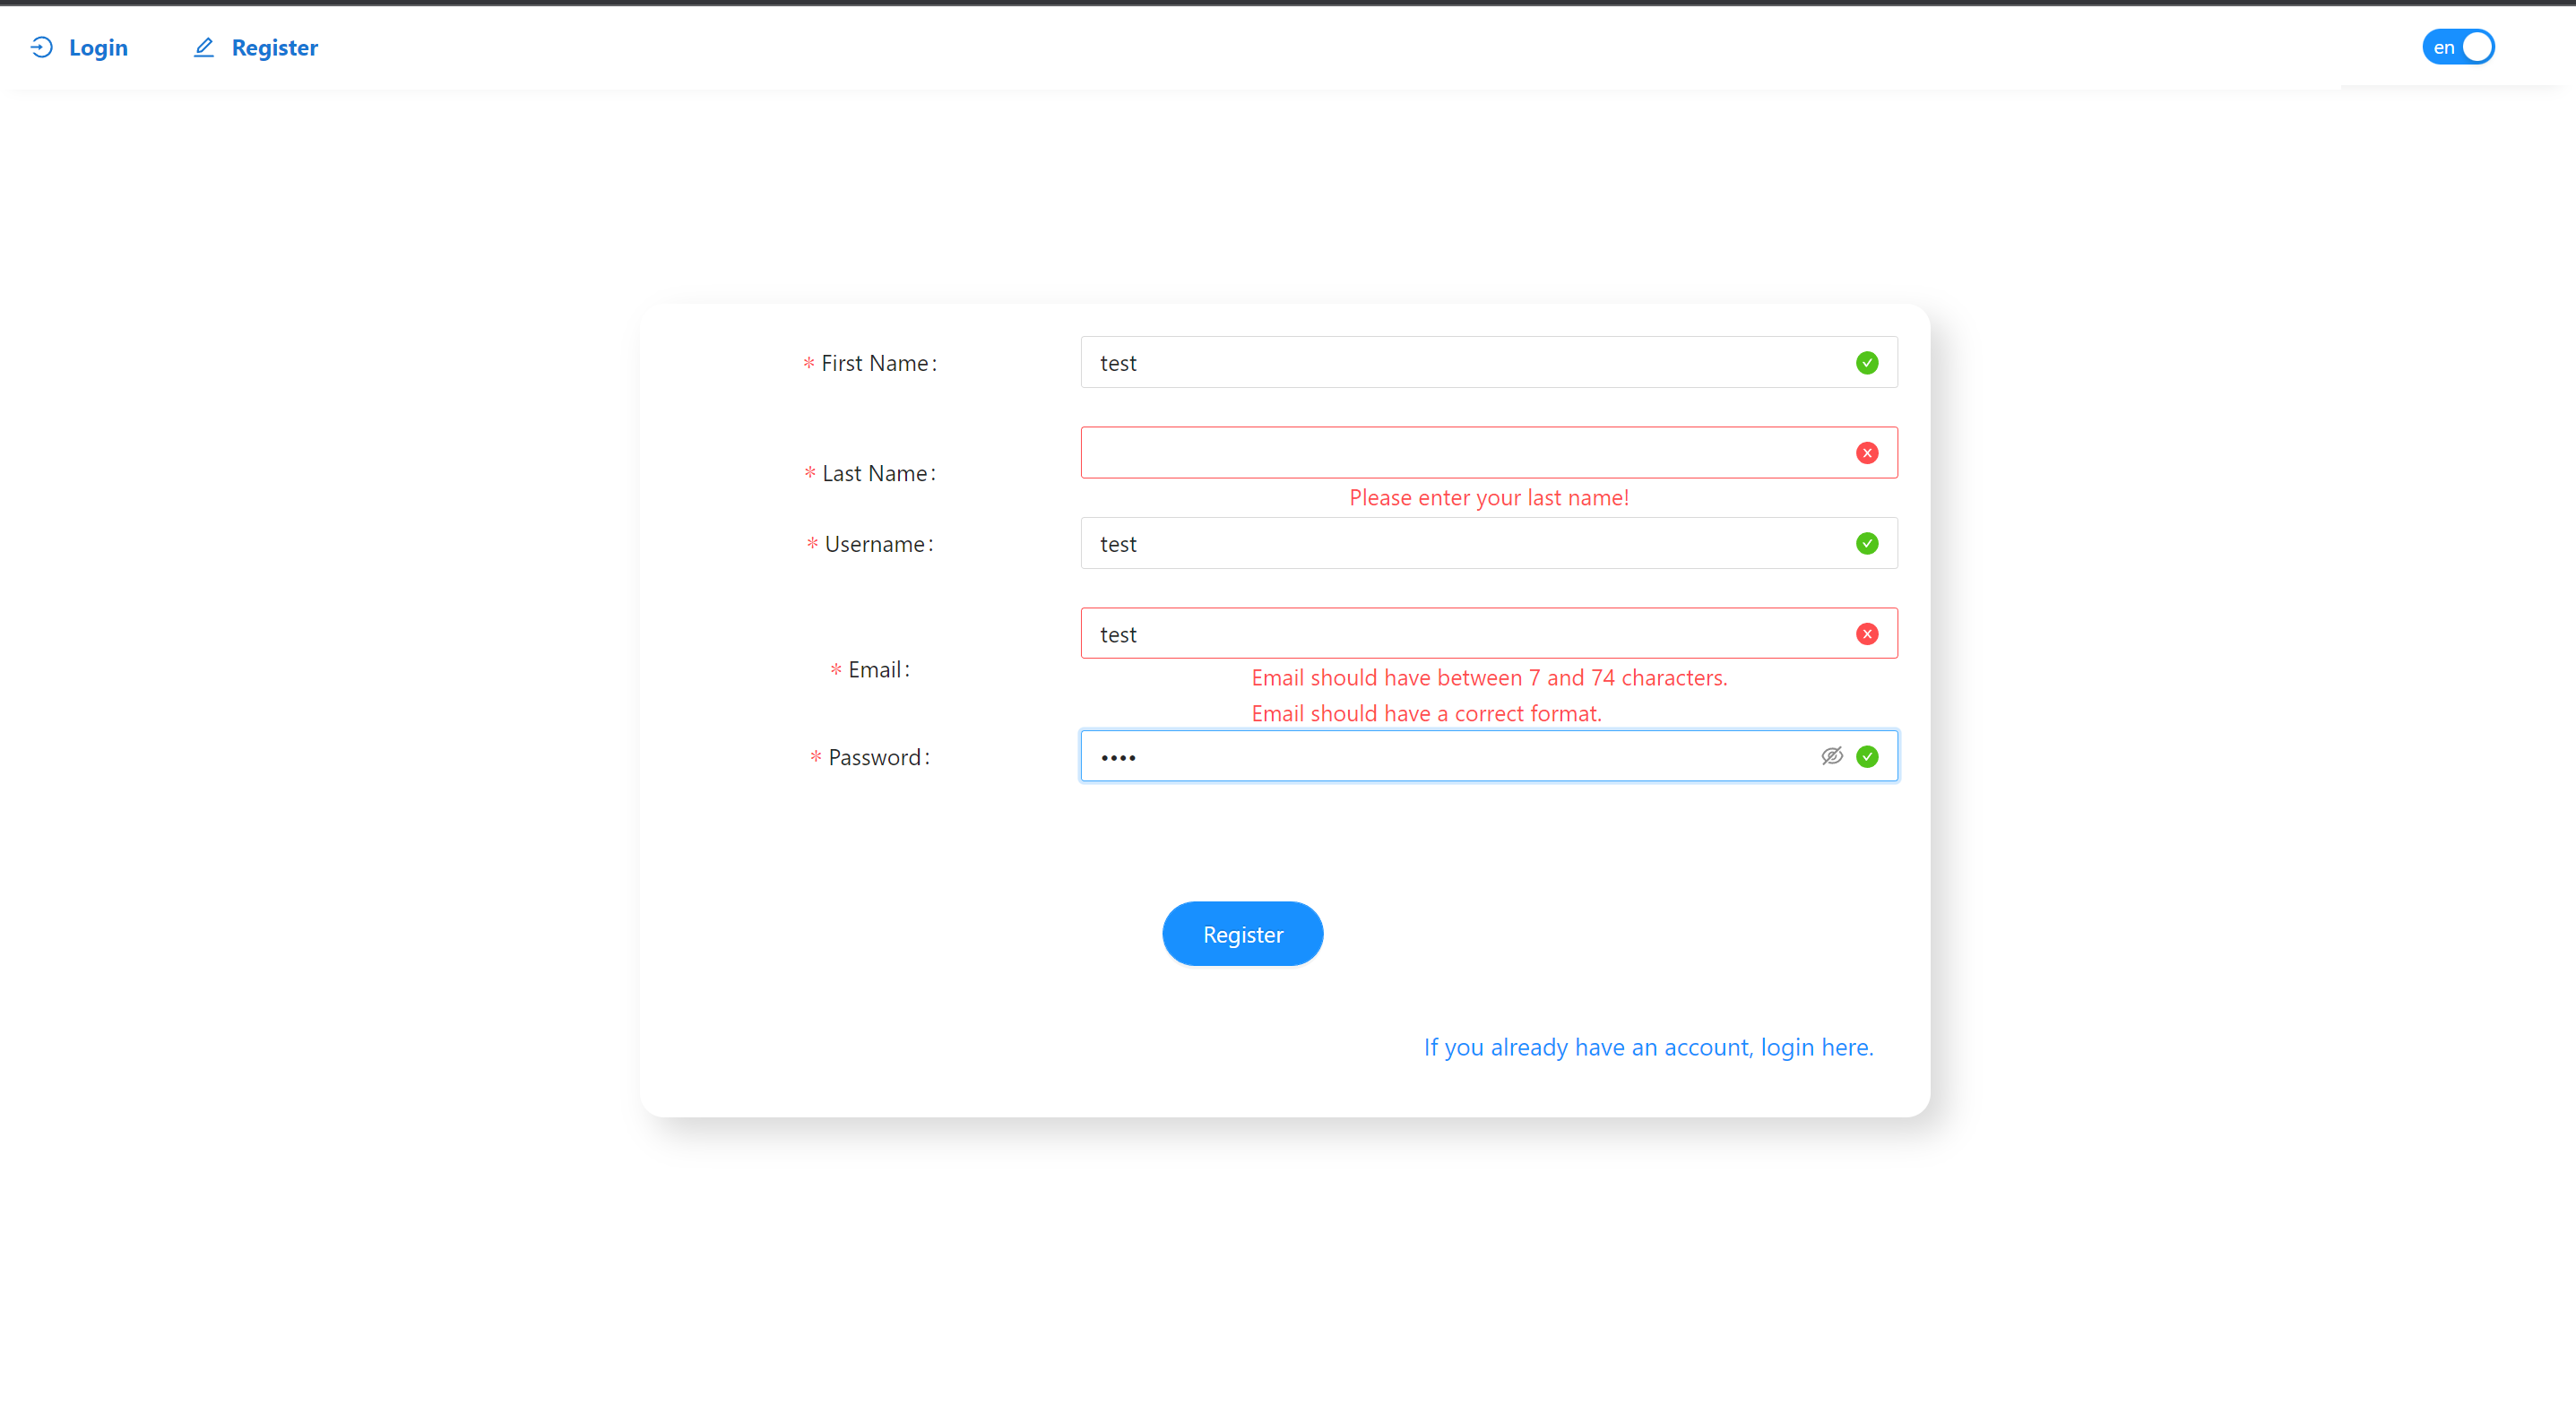
\includegraphics[width=150mm]{figs/createAccount.png}
    \caption{Pagina de creare cont nou}
	\label{fig:createAccount}
\end{figure}

După ce contul a fost creat cu succes, se ajunge la pagina de login, unde trebuie completate credențialele pentru a putea intra în aplicație. 
În cazul în care credențialele nu sunt corecte, utilizatorul va fi notificat, după cum se poate vedea în figura \ref{fig:wrongCredentialsLogin}. 
\begin{figure}[H]
	\centering
	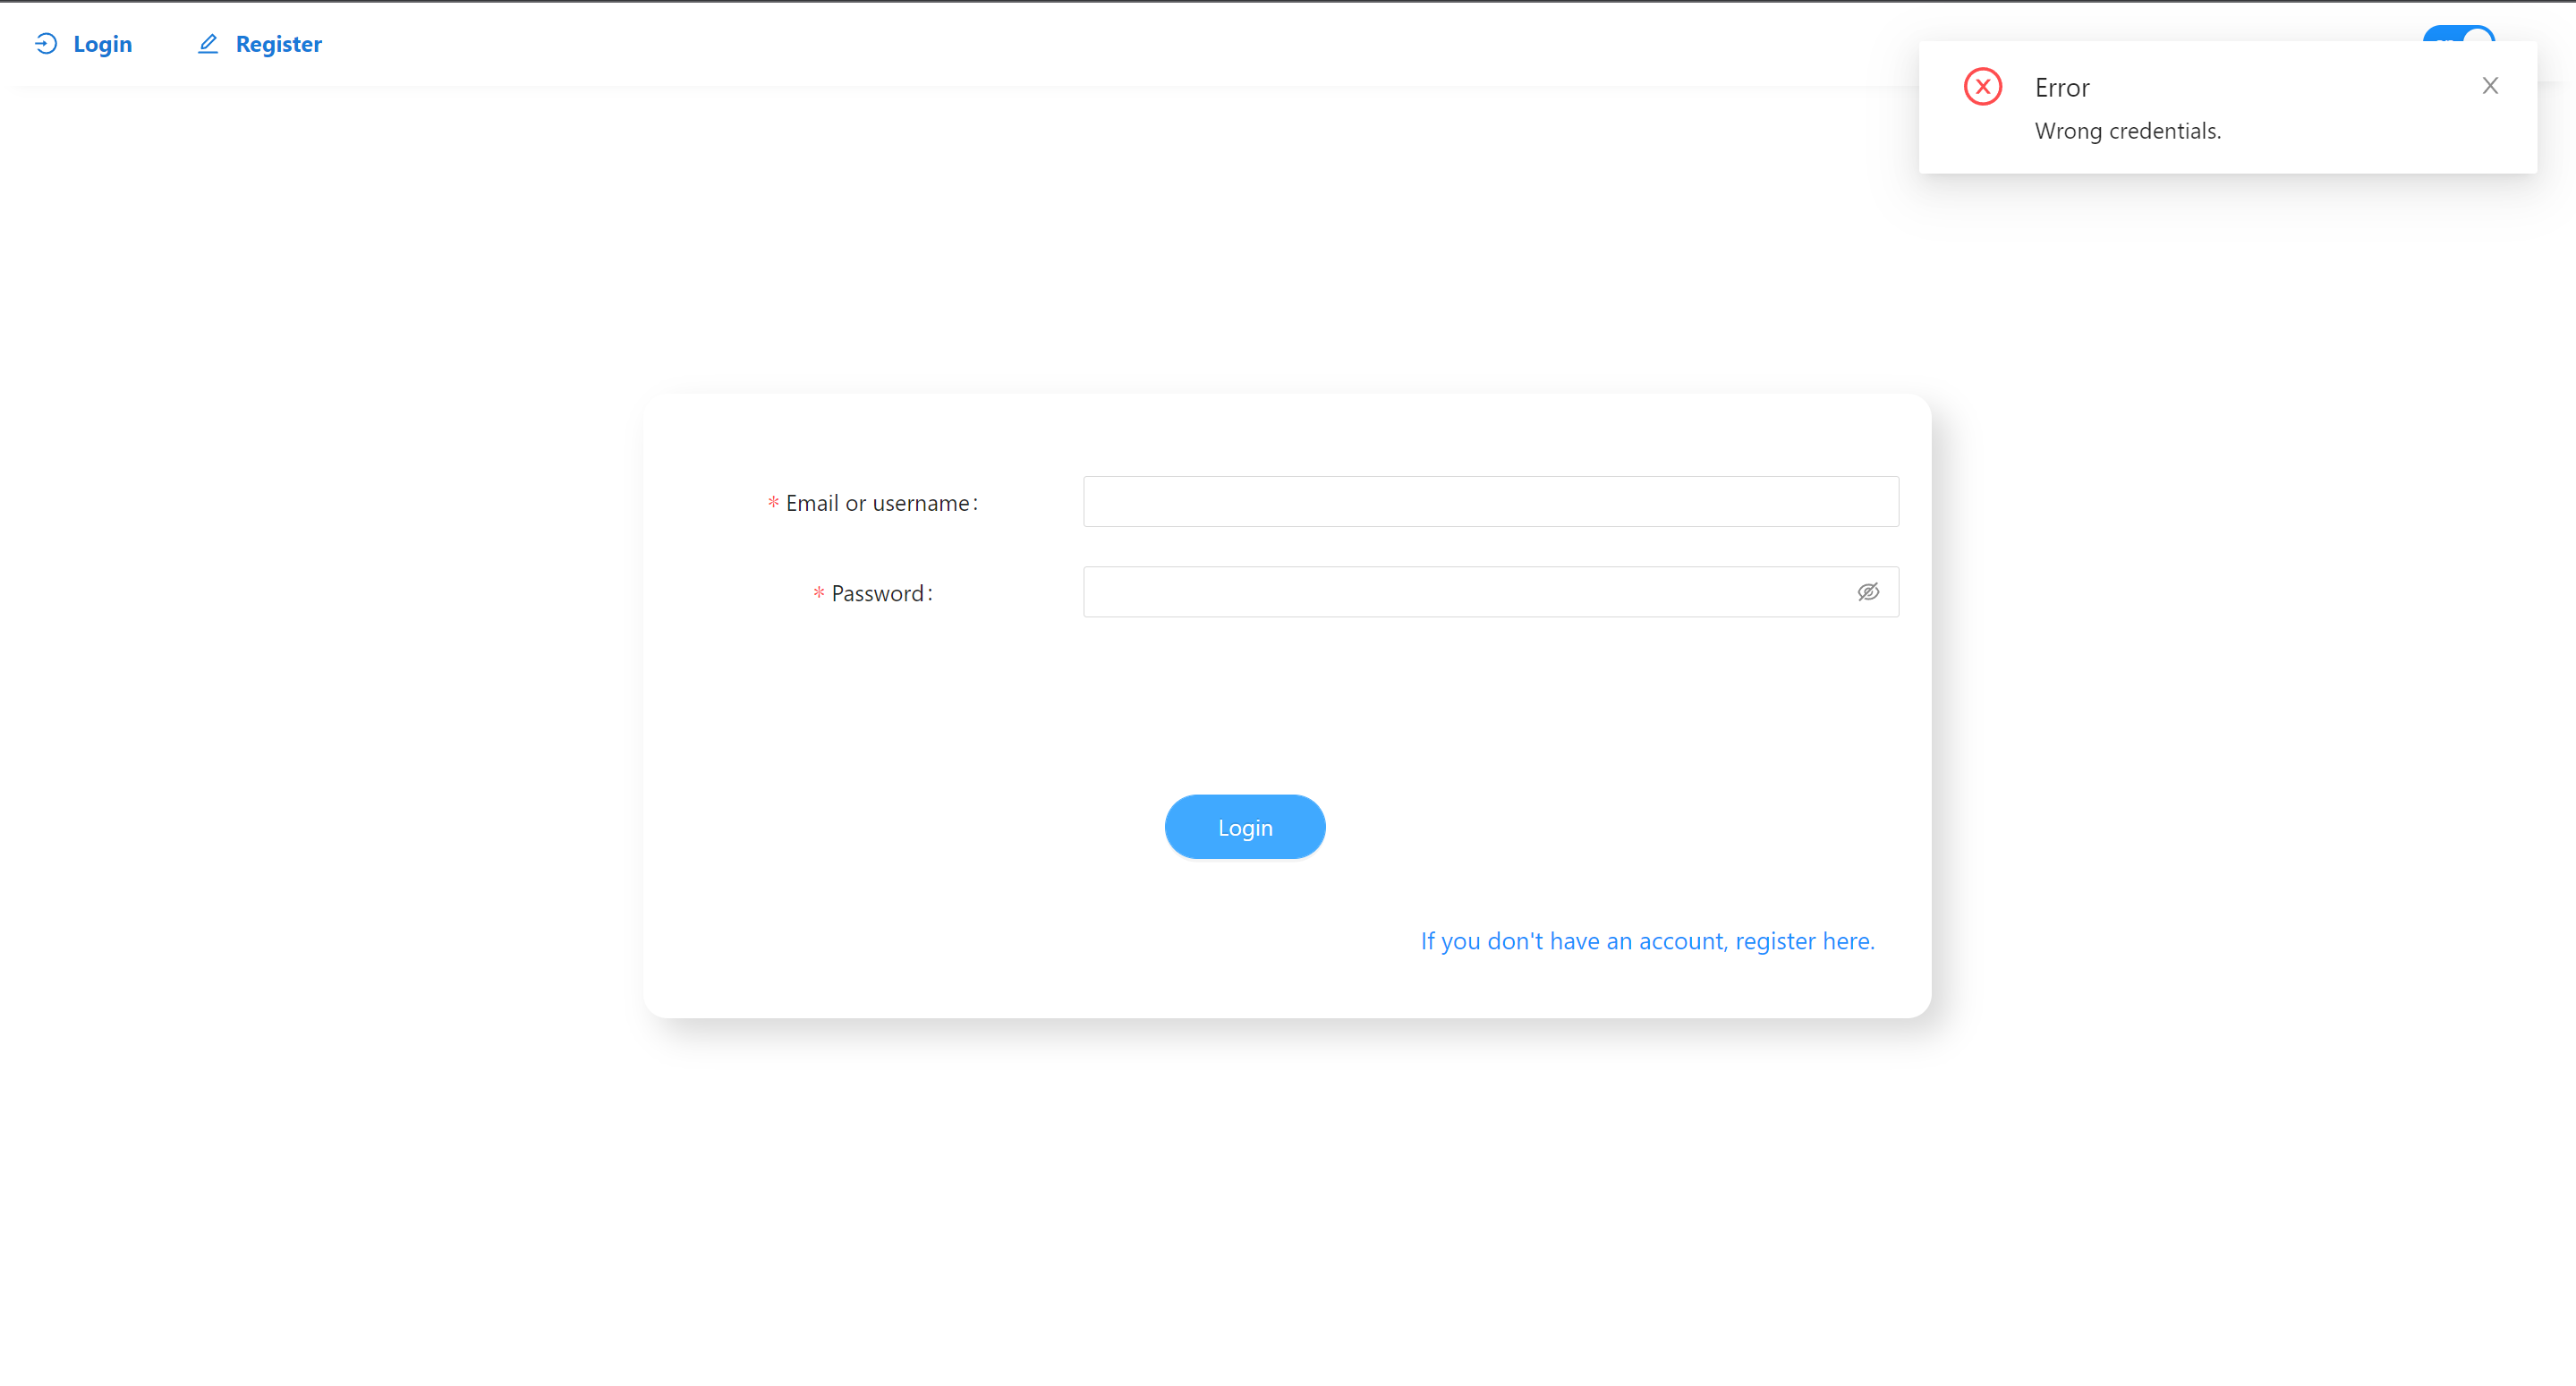
\includegraphics[width=150mm]{figs/wrongCredentialsLogin.png}
    \caption{Credențiale greșite la logarea în aplicație}
	\label{fig:wrongCredentialsLogin}
\end{figure}
În acest moment, utilizatorul nu este logat și are acces doar la pagina de Login și pagina de Register, toate celelalte pagini din aplicație sunt inaccesibile, iar daca va încerca să ajungă la una din ele din URL, 
acesta va fi redirecționat automat la pagina de login. 

Când credențialele corecte au fost completate, utilizatorul va intra în aplicație. În acest moment, are acces la toate paginile și resursele din aplicație, dar nu are acces la paginile de Login și Register. 

După logare, pe pagina de Dashboard, utilizatorul poate adauga în caseta de text un text pe care dorește să îl analizeze. Nu poate trece mai departe, la componentele de afișare a informațiilor detaliate
până când nu există input în casetă; altfel, va primi un mesaj specific, cum e în figura \ref{fig:dashboardInput}.
\begin{figure}[H]
	\centering
	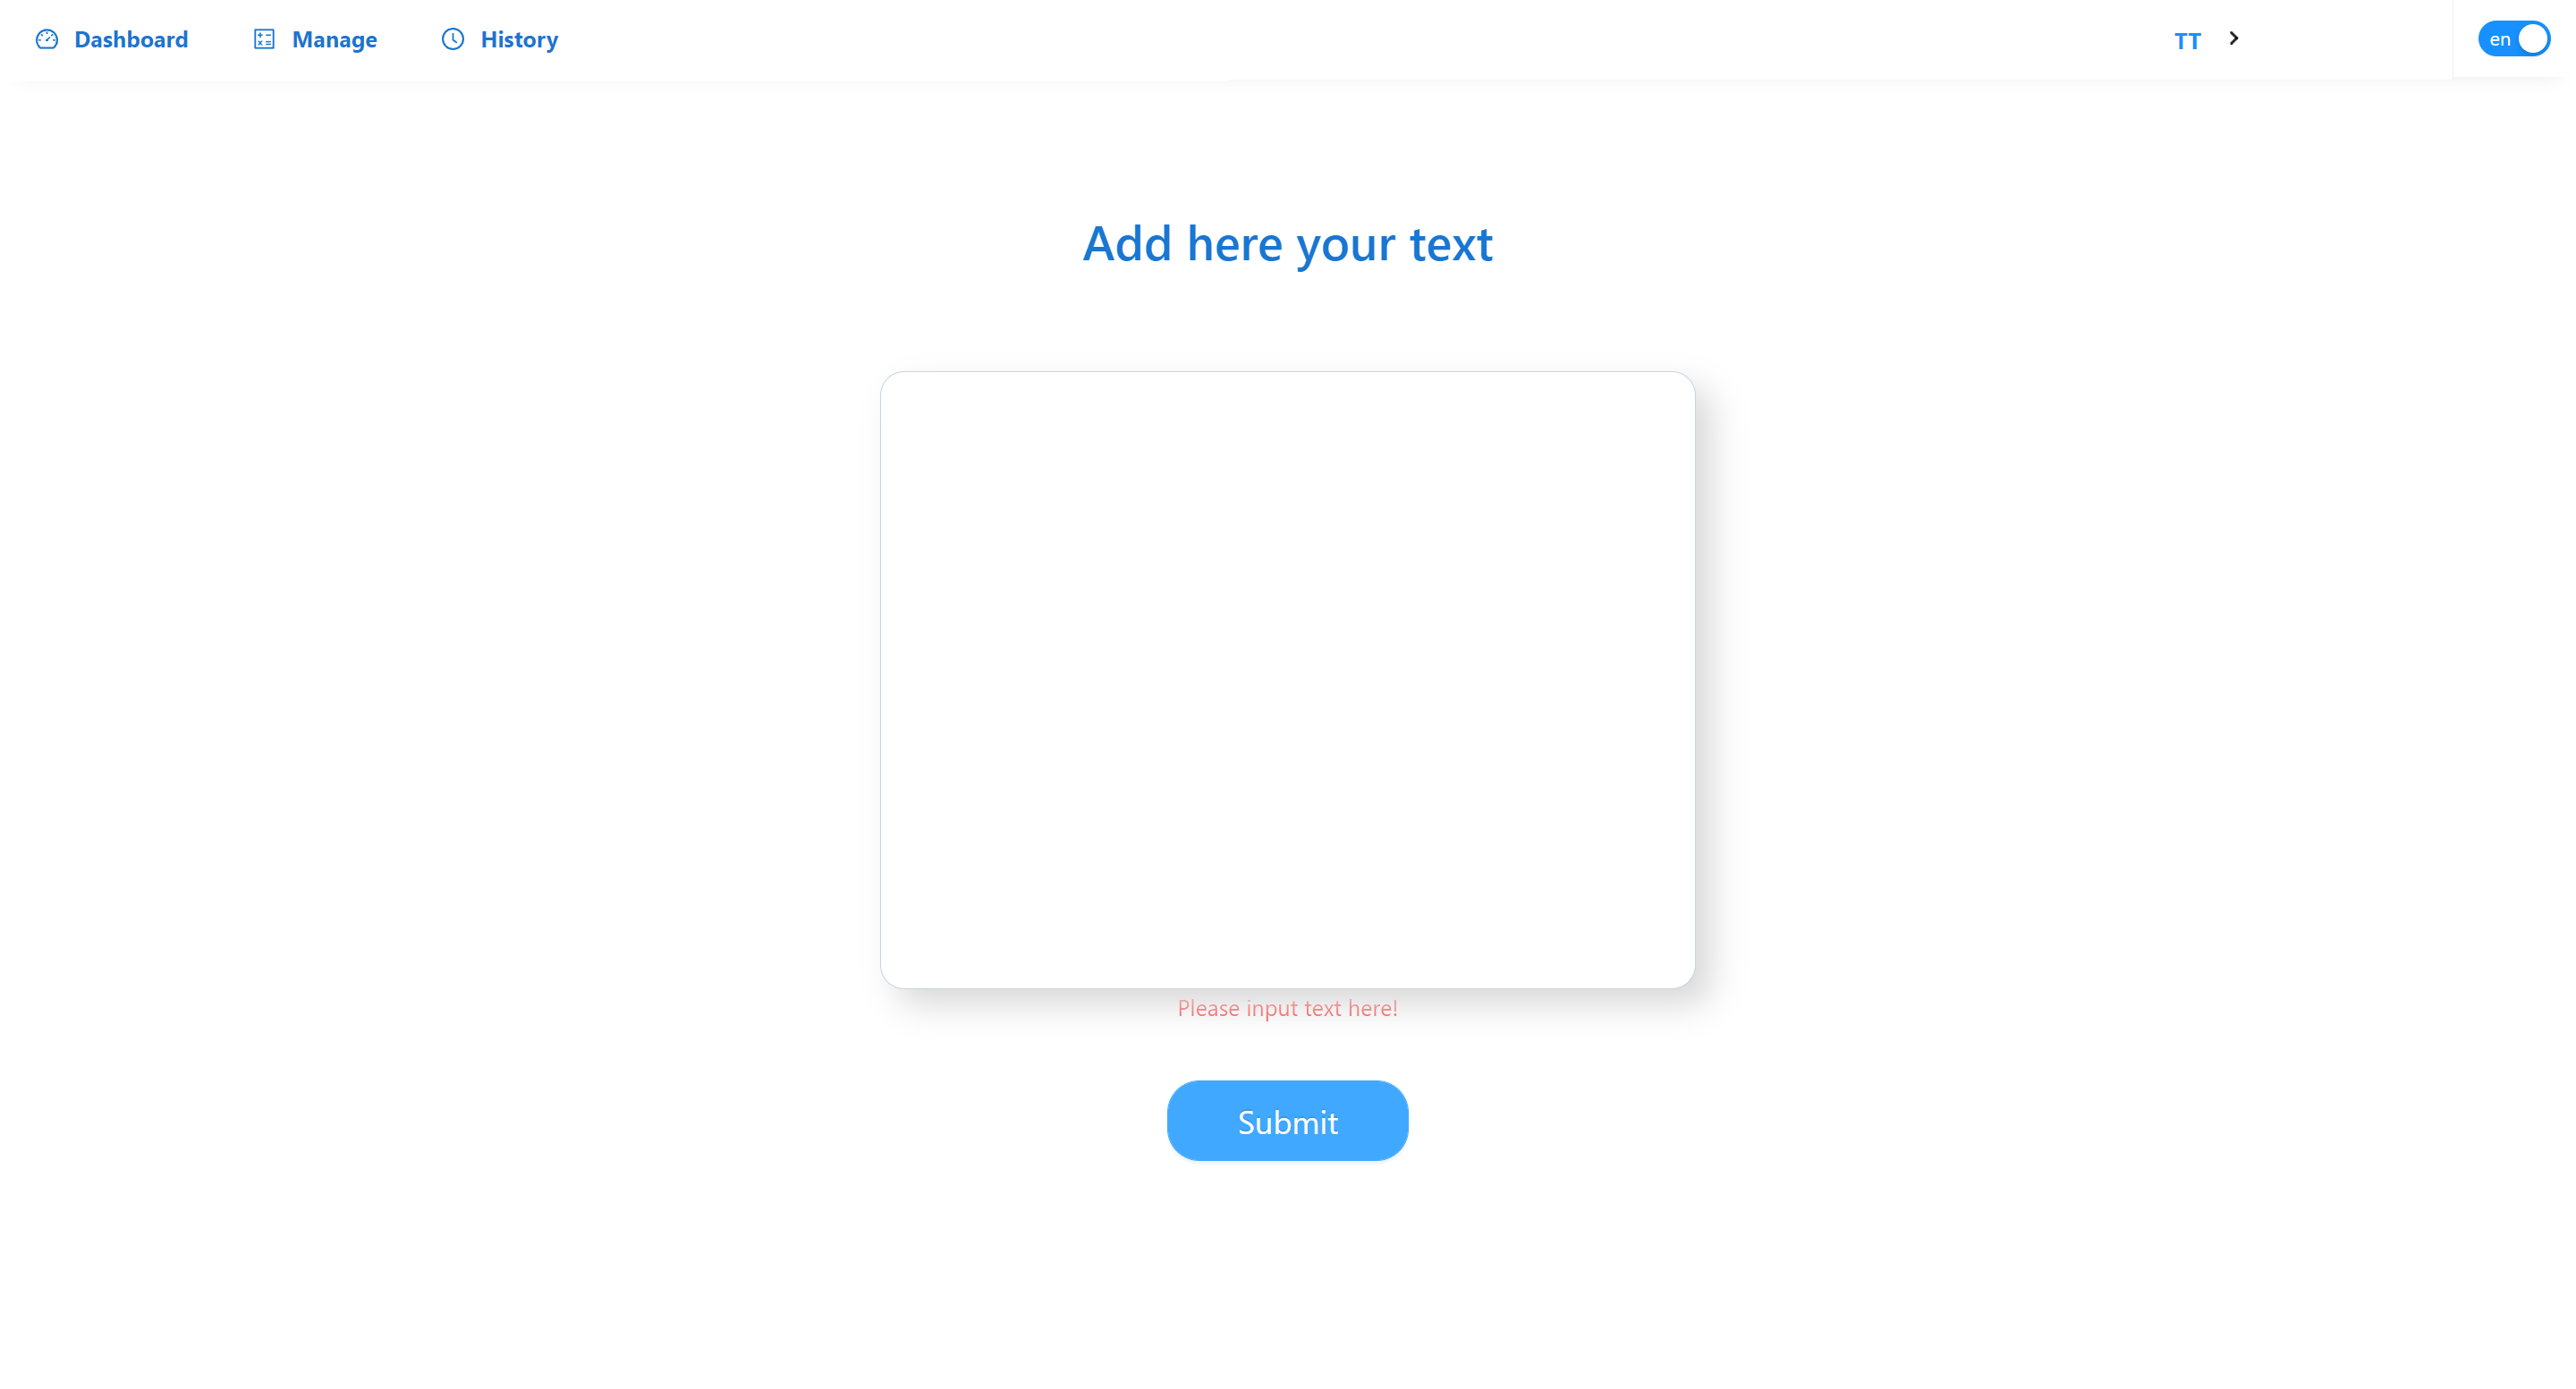
\includegraphics[width=150mm]{figs/dashboardInput.png}
    \caption{Încercare de a efectua o analiză fără input de la utilizator}
	\label{fig:dashboardInput}
\end{figure}

După ce userul a adăugat textul pe care dorește să îl analizeze și apasă pe butonul SUBMIT, rezultatele vor apărea și un buton de mers la următoarea pagină se va încărca, cum apare în figura \ref{fig:seeMoreButton}.
\begin{figure}[H]
	\centering
	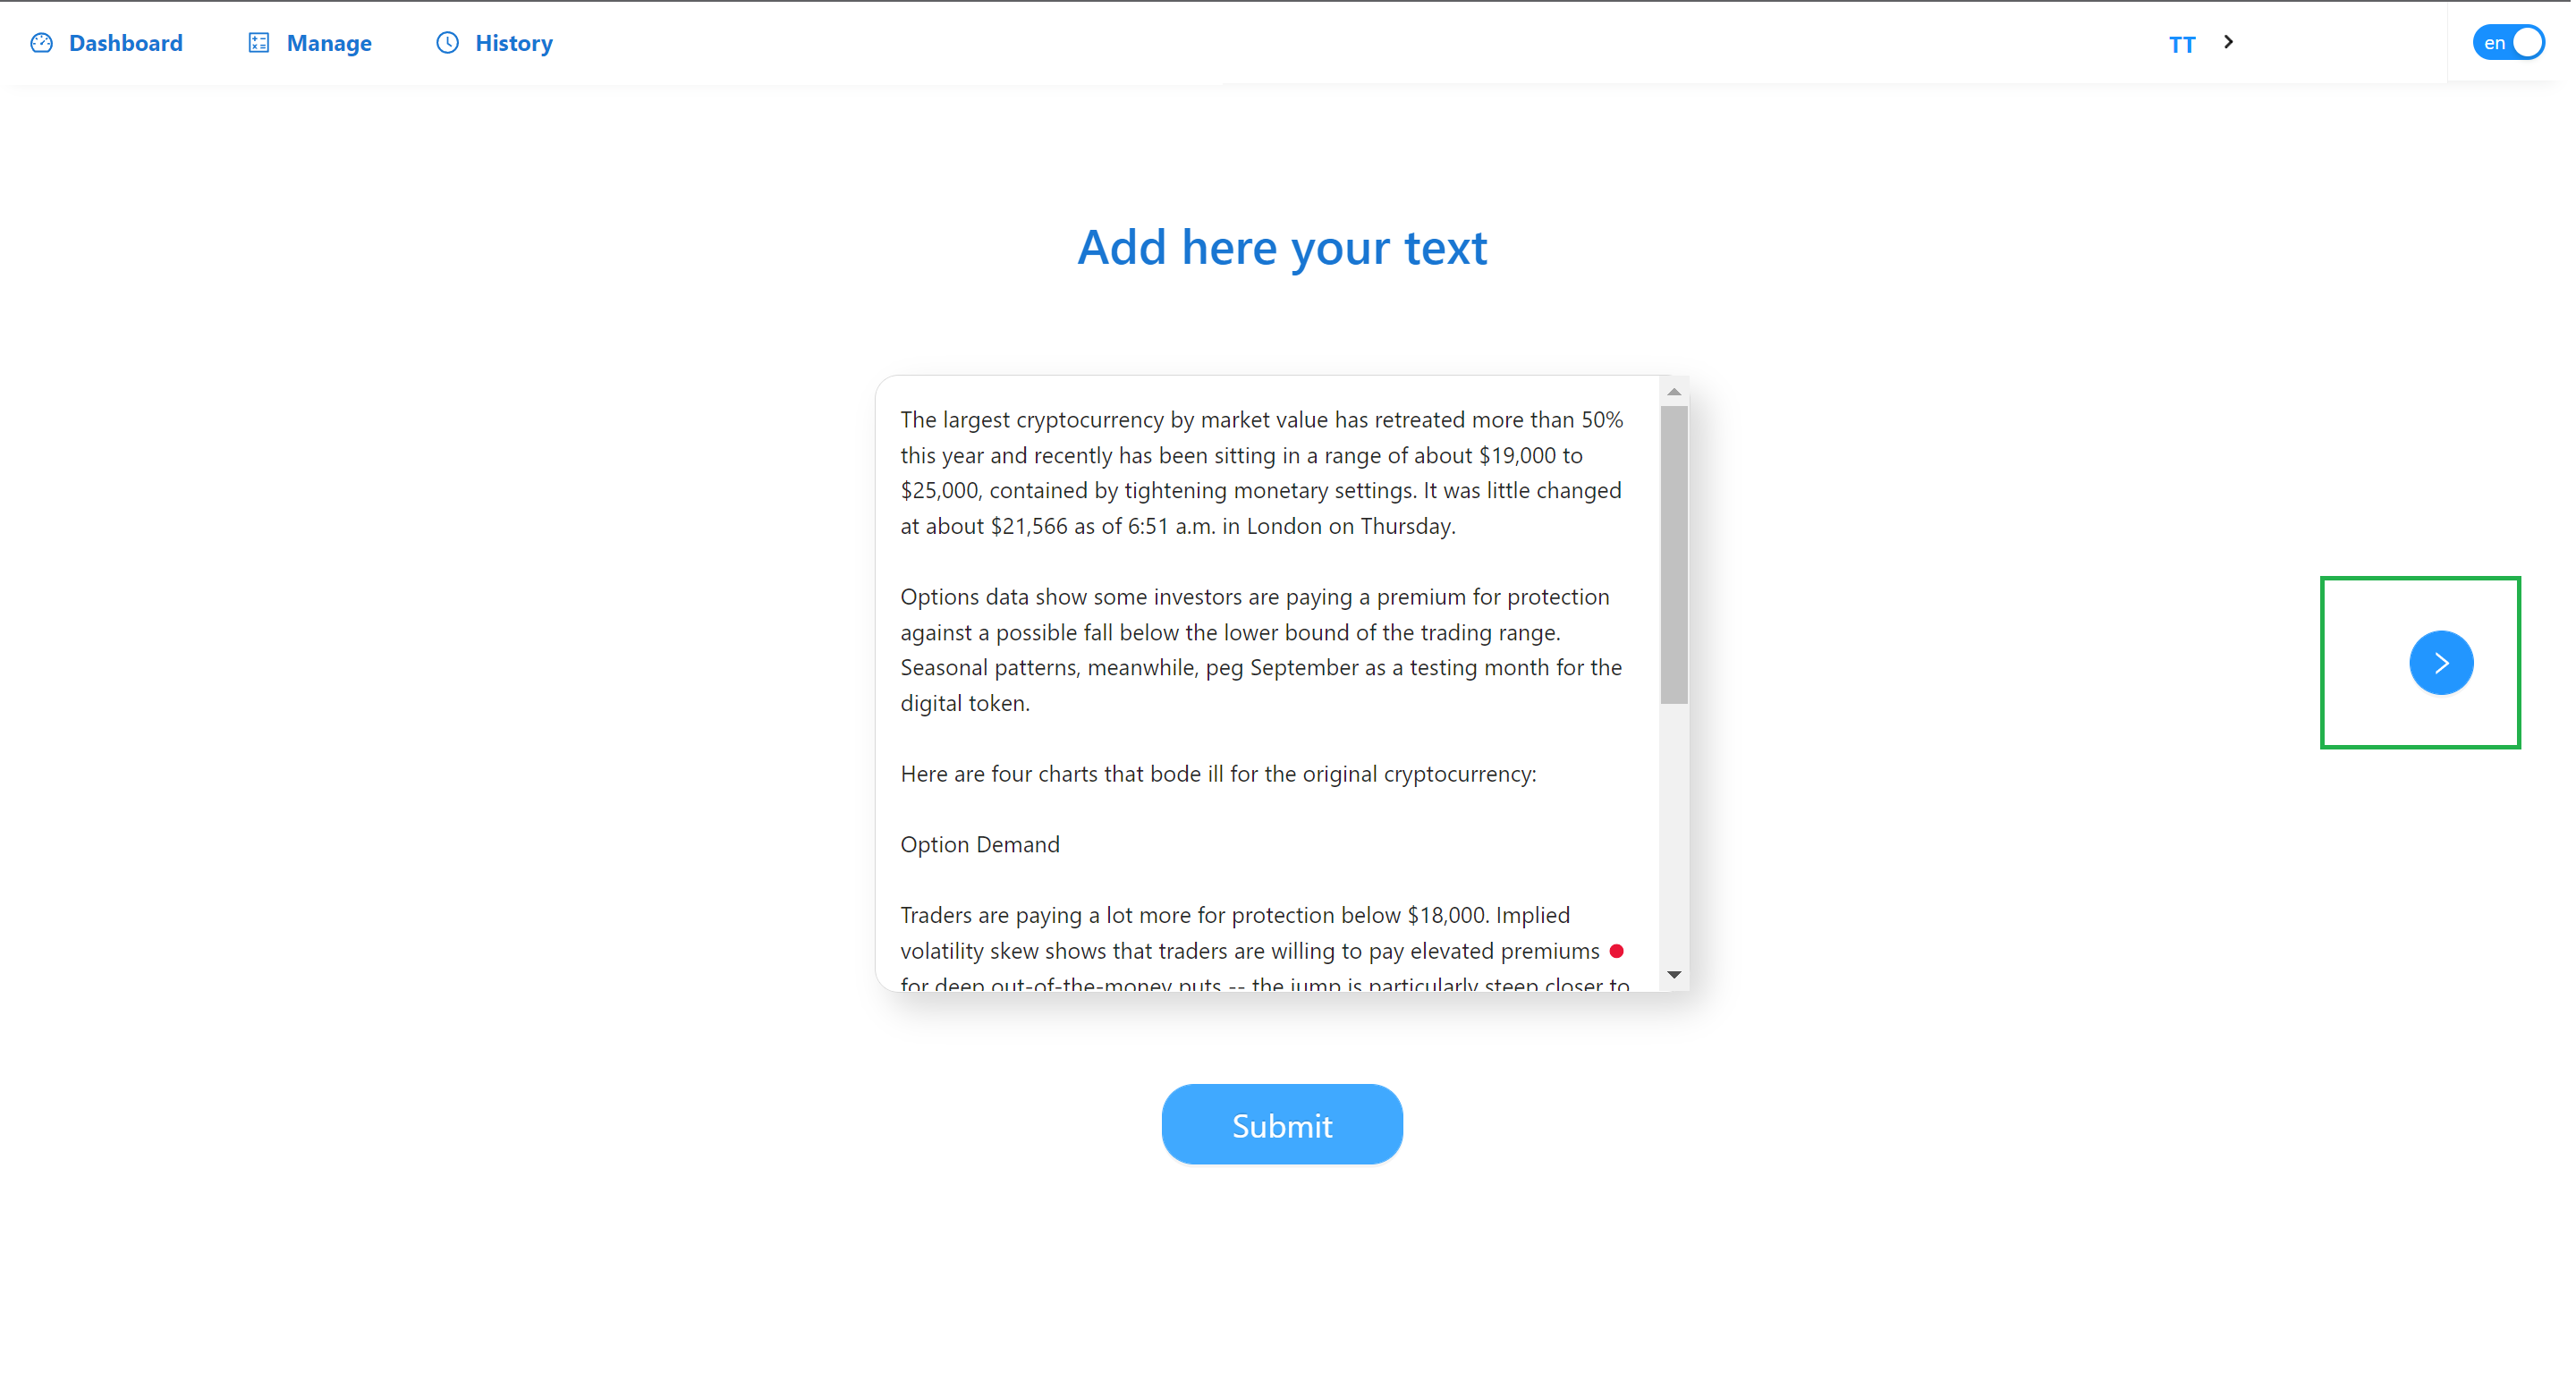
\includegraphics[width=150mm]{figs/seeMoreButton.png}
    \caption{Buton pentru a merge în pagina de vizualizare a analizei detaliate a textului}
	\label{fig:seeMoreButton}
\end{figure}

După ce ajungem în pagina cu informații detaliate despre textul analizat, putem observa pe primul rând 2 carduri în care este afișat textul original și textul sumarizat. \\
În următorul card, avem statisticile sentimentelor - pozitiv, neutru și negativ. Aceste informații se pot vedea în figura \ref{fig:seeMore1}.
\begin{figure}[H]
	\centering
	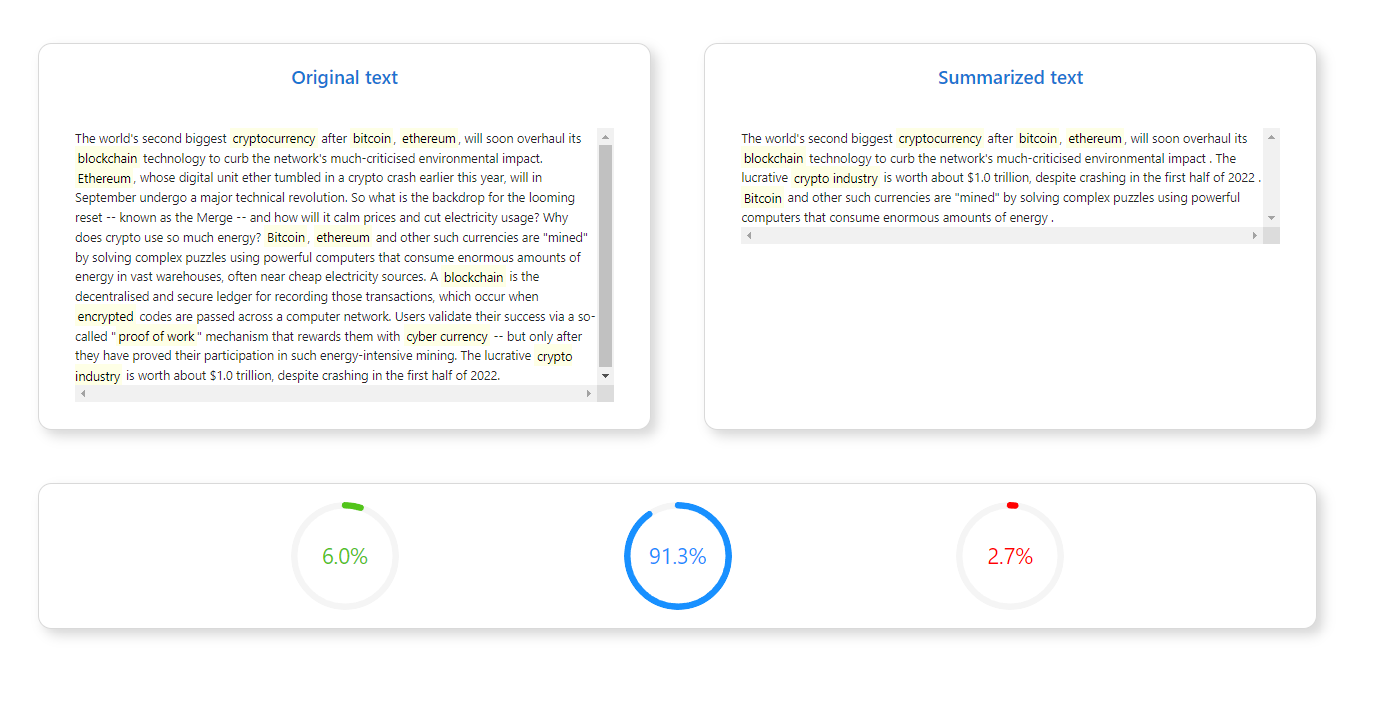
\includegraphics[width=150mm]{figs/seeMore1.png}
    \caption{Rezultate analiza - partea 1}
	\label{fig:seeMore1}
\end{figure}

În ultimul card, care este unul interactiv, utilizatorul poate alege dintre cuvintele cheie extrase din text și perioada dorită pentru a genera graficul aparițiilor, după cum se poate vedea în figura \ref{fig:seeMore2}. \\
În acest grafic, în primul dropdown sunt cuvintele cheie extrase din text. Acestea pot fi observate fiind evidențiate prin subliniere în textul original din figura \ref{fig:seeMore1}. 
Rezultatul pe grafic poate fi observat în figura \ref{fig:keywordsEvolution}.

\begin{figure}[H]
	\centering
	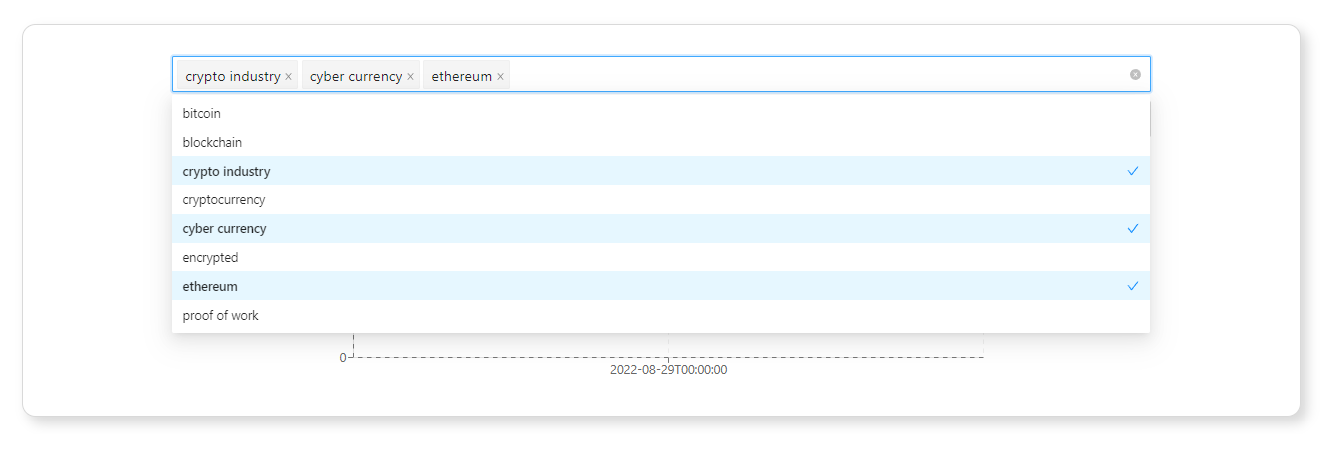
\includegraphics[width=150mm]{figs/seeMore2.png}
    \caption{Rezultate analiza - partea 2}
	\label{fig:seeMore2}
\end{figure}
\begin{figure}[H]
	\centering
	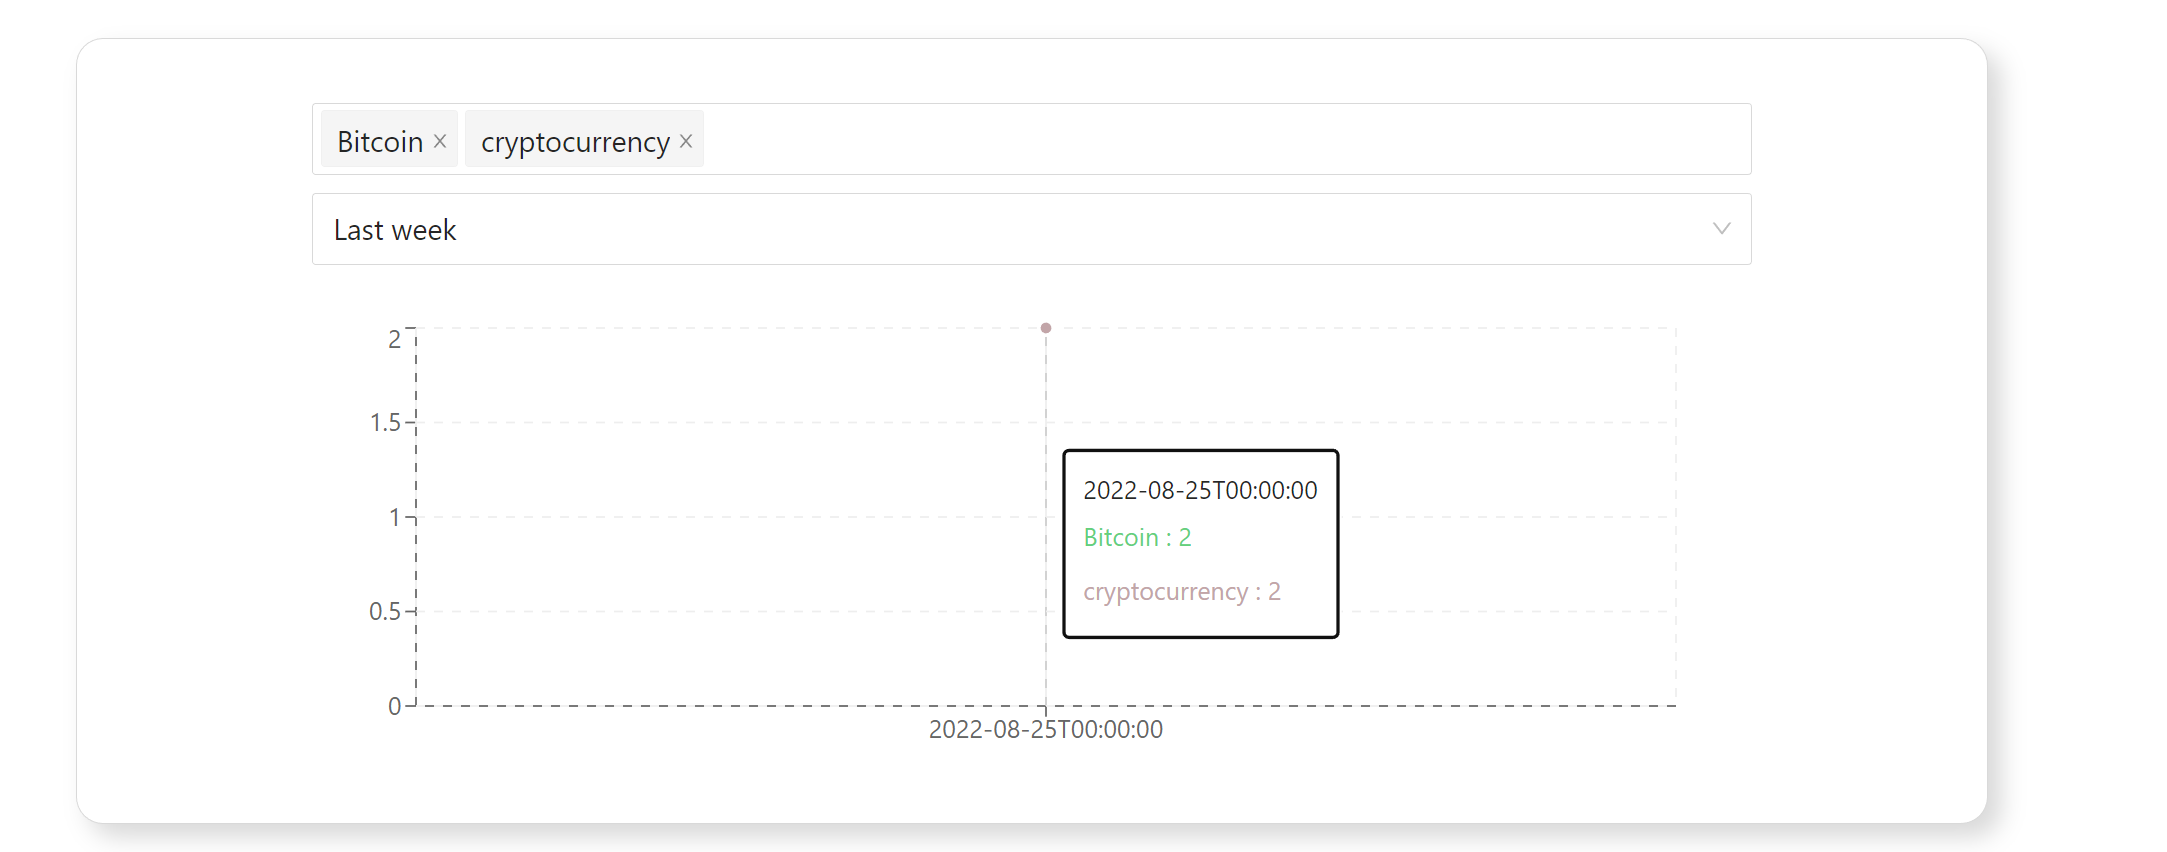
\includegraphics[width=150mm]{figs/keywordsEvolution.png}
    \caption{Rezultate analiza - evoluție cuvinte cheie}
	\label{fig:keywordsEvolution}
\end{figure}

În acest punct, se poate observa butonul de salvare a articolului analizat, împreună cu rezultatele obținute în istoricul personal al utilizatorului, în figura \ref{fig:saveArticle}.  \\
Informațiile pot fi redeschise ulterior, în orice moment, din pagina de Dashboard, cum apar în figura \ref{fig:personalHistory}, apăsând butonul See More. De asemenea, articolele pot fi șterse din istoricul personal
al utilizatorului apăsând butonul Delete.
\begin{figure}[H]
	\centering
	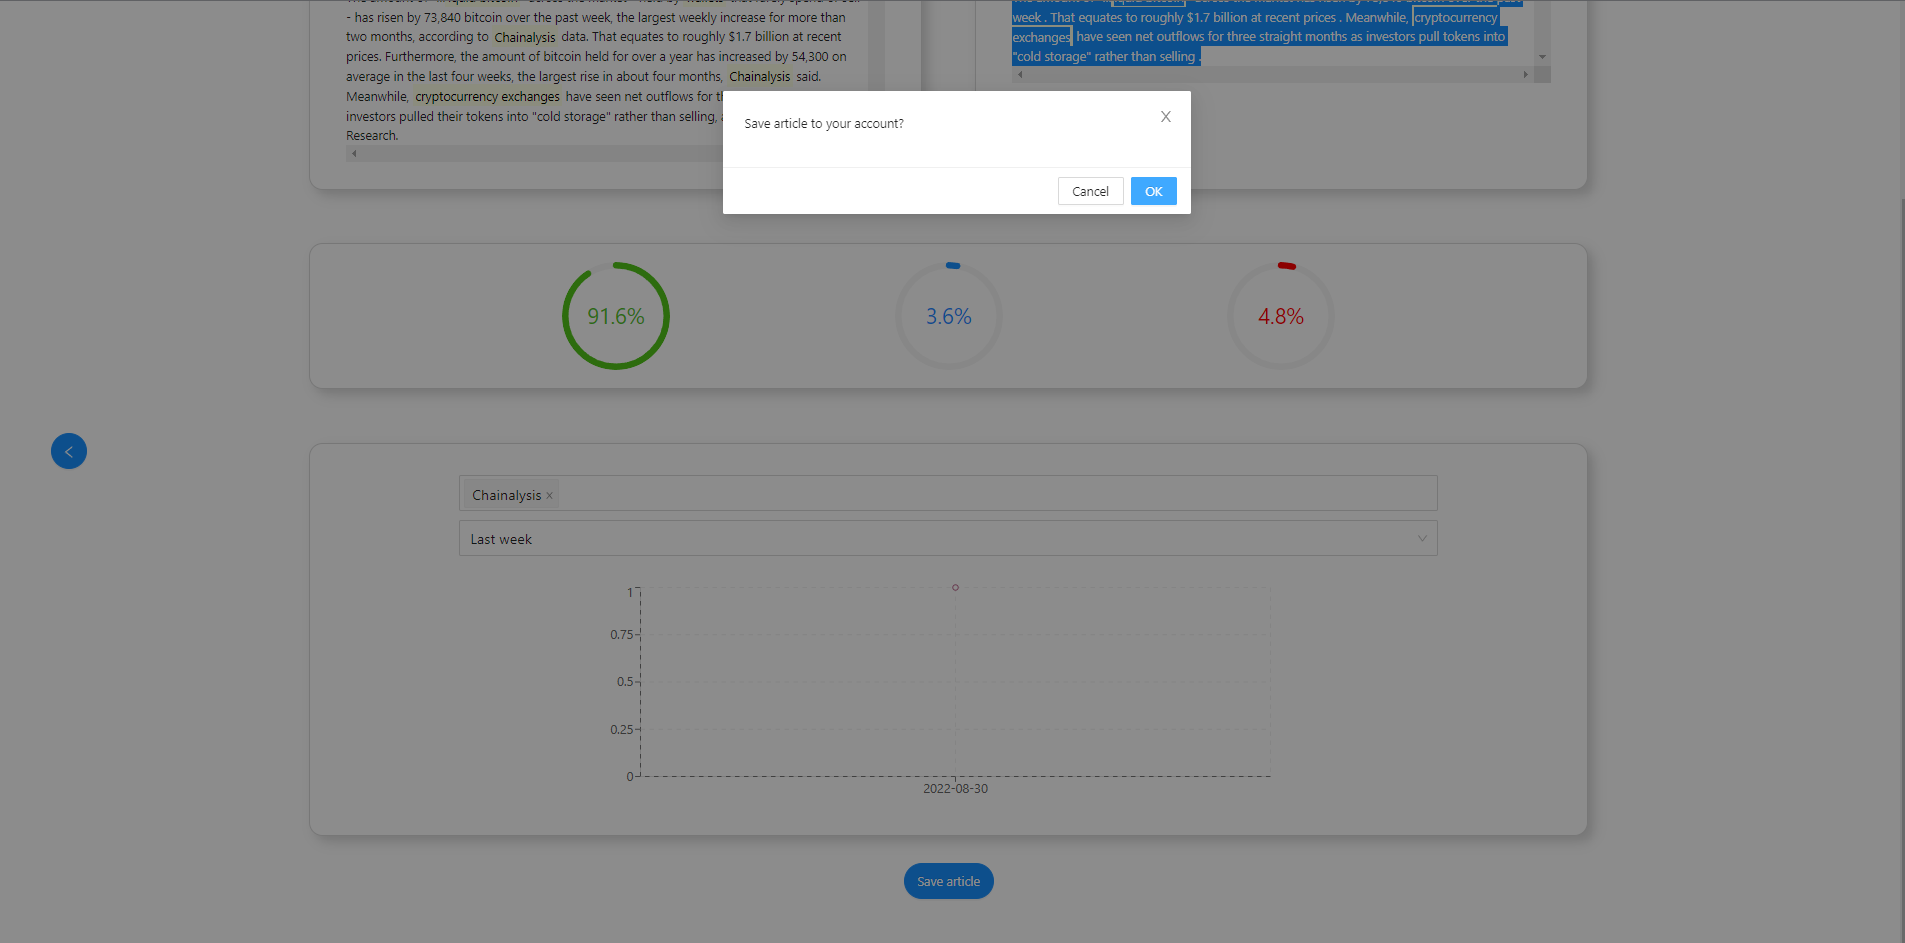
\includegraphics[width=150mm]{figs/saveArticle.png}
    \caption{Buton de salvare articol}
	\label{fig:saveArticle}
\end{figure}
\begin{figure}[H]
	\centering
	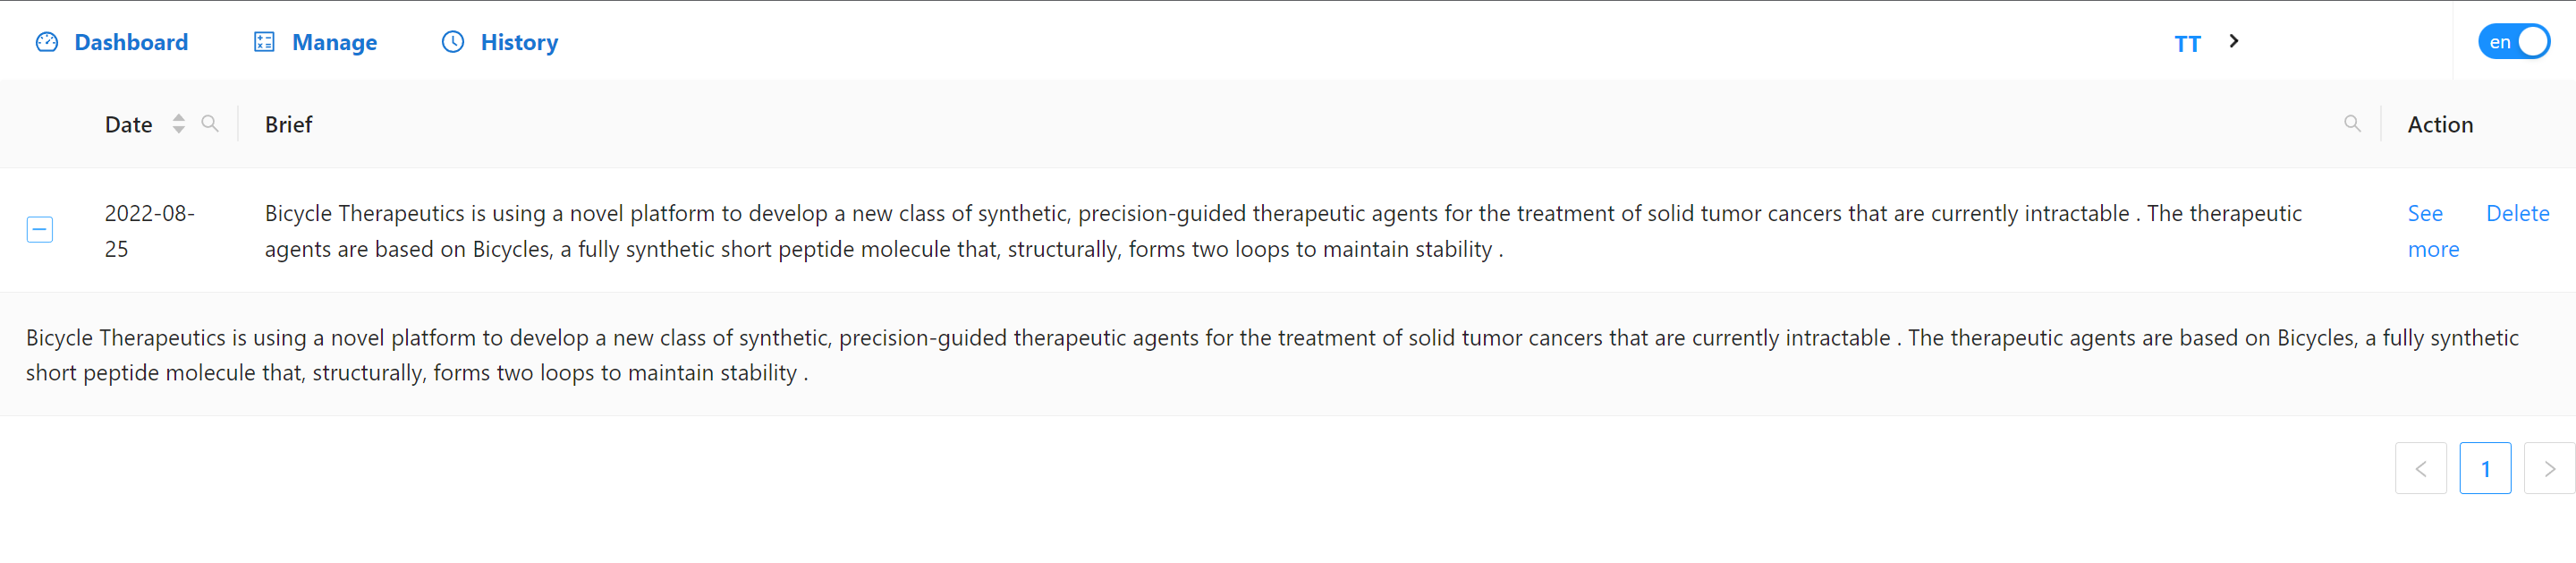
\includegraphics[width=150mm]{figs/personalHistory.png}
    \caption{Istoricul analizelor de text salvate de utilizator}
	\label{fig:personalHistory}
\end{figure}

Pentru a edita informațiile contului utilizatorul, se accesează pagina de Profile. Câmpurile care pot fi modificate sunt Nume, Prenume, Nume de utilizator, Email, Parola. 
Singurele restricții în modificarea acestor câmpuri sunt ca Numele de utilizator și Email-ul să fie unice, neatribuite altui cont existent, altfel utilizatorul va fi notificat cu una dintre următoarele erori, ca în figura \ref{fig:editProfileUsername}.

\begin{figure}[H]
	\centering
	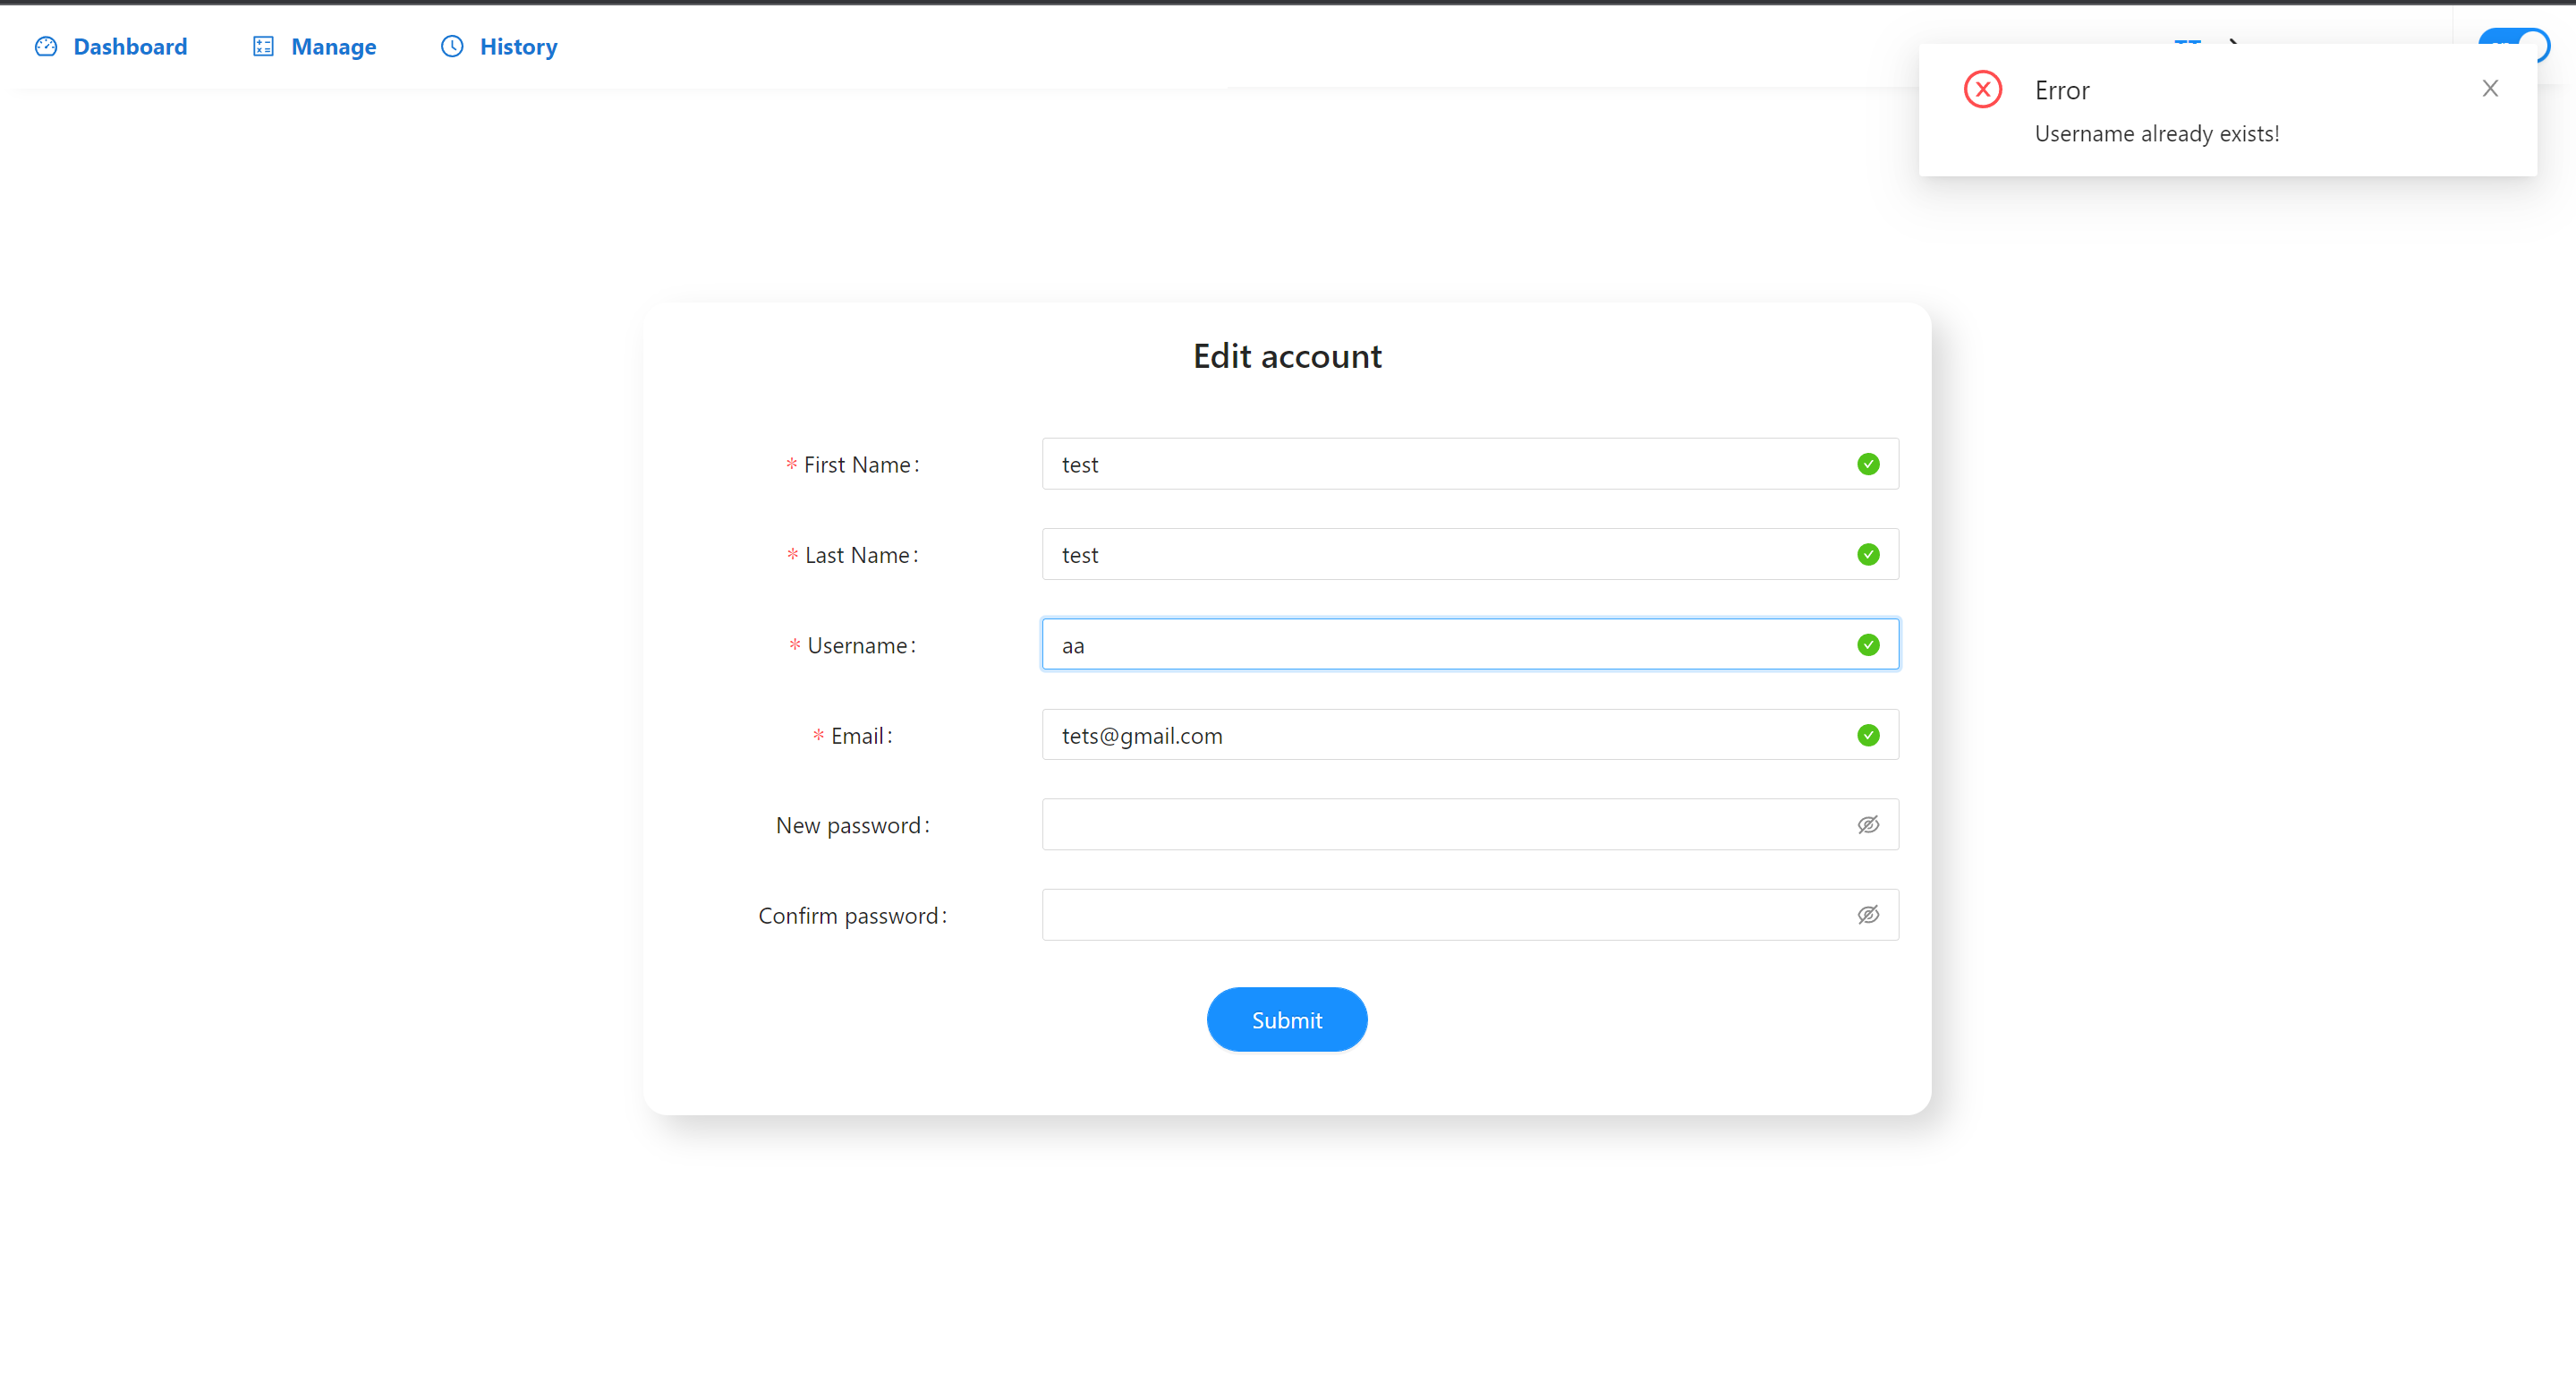
\includegraphics[width=150mm]{figs/editProfileUsername.png}
    \caption{Utilizatorul încearcă să își schimbe username-ul, dar acesta este deja atribuit altui cont}
	\label{fig:editProfileUsername}
\end{figure}

După ce utilizator a ales un nou username și/sau email care respectă condiția de unicitate, acesta va fi notificat că actualizarea detaliilor contului s-a făcut cu succes, cum apare în figura \ref{fig:editProfile}.
\begin{figure}[H]
	\centering
	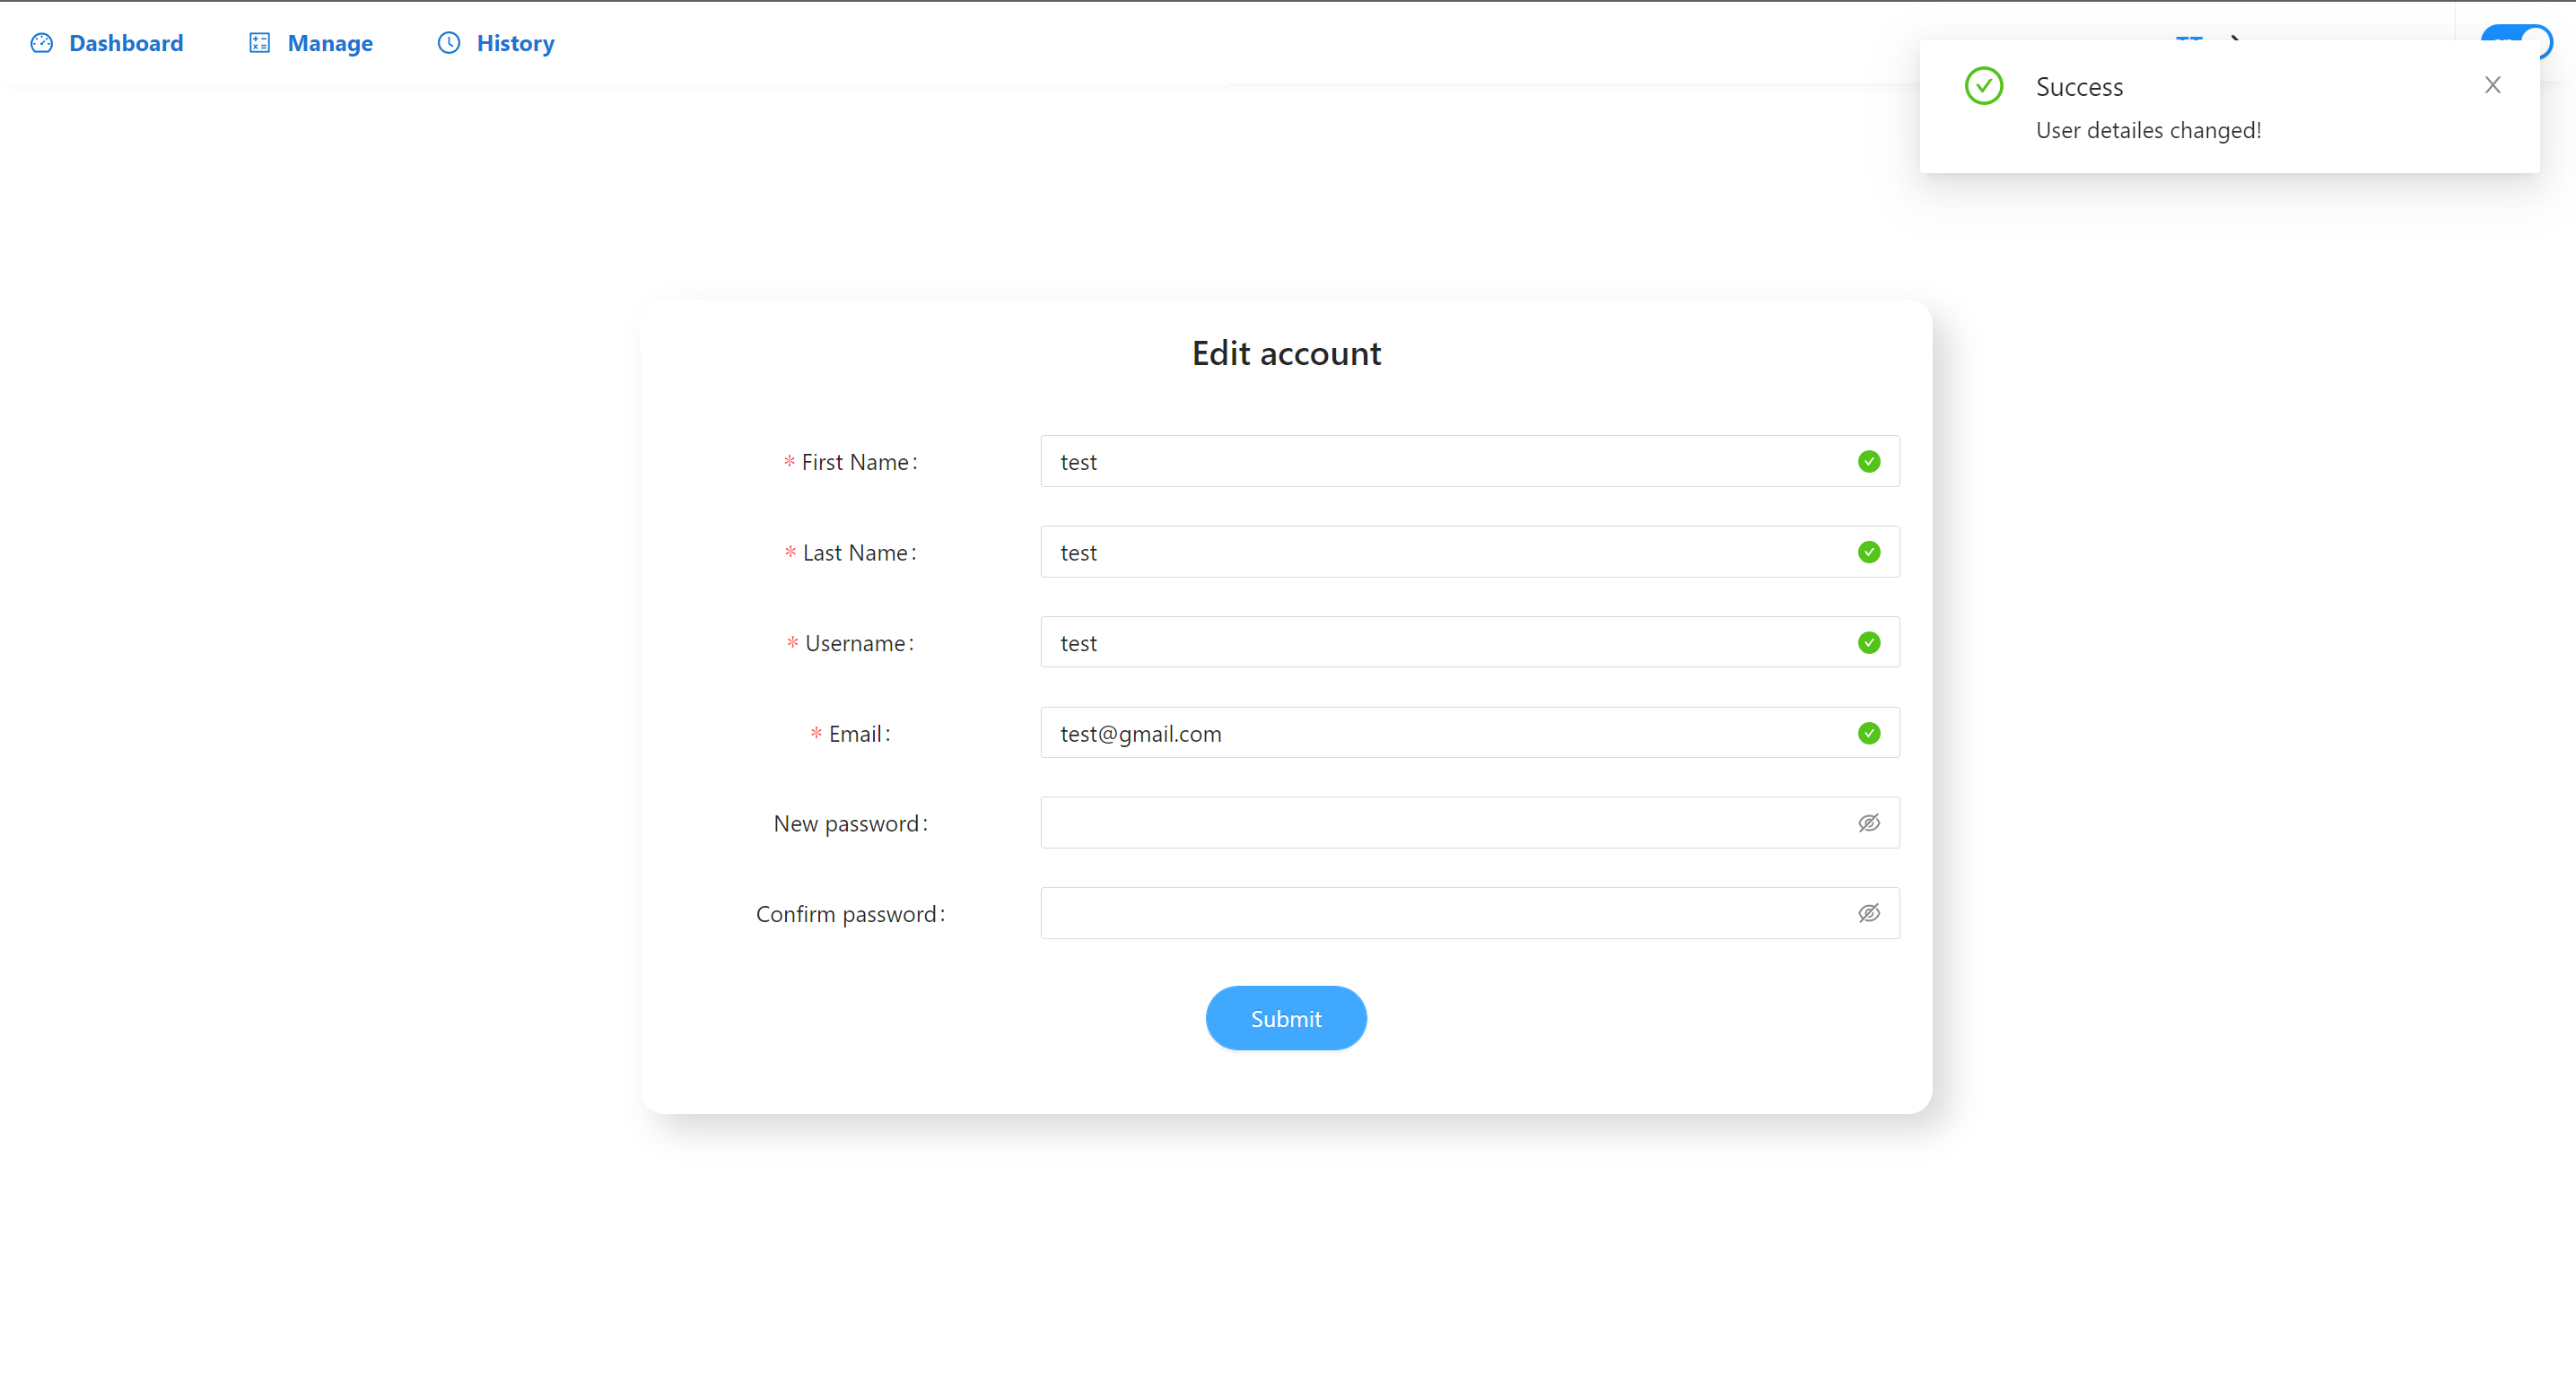
\includegraphics[width=150mm]{figs/editProfile.png}
    \caption{Actualizare detalii cont cu succes}
	\label{fig:editProfile}
\end{figure}

În pagina de Manage, utilizatorul poate vedea topicele cele mai populare, adică cele mai des apărute cuvinte cheie sau expresii în analizele efectuate și de restul utilizatorilor.\\
În cazul în care utilizatorul a selectat o perioadă în care nu sunt înregistrate date, va fi notificat de acest lucru, ca în figura \ref{fig:trendingNoData}, altfel rezultatele vor fi afișate pe grafic, ca în figura \ref{fig:trending}. 
\begin{figure}[h]
	\centering
	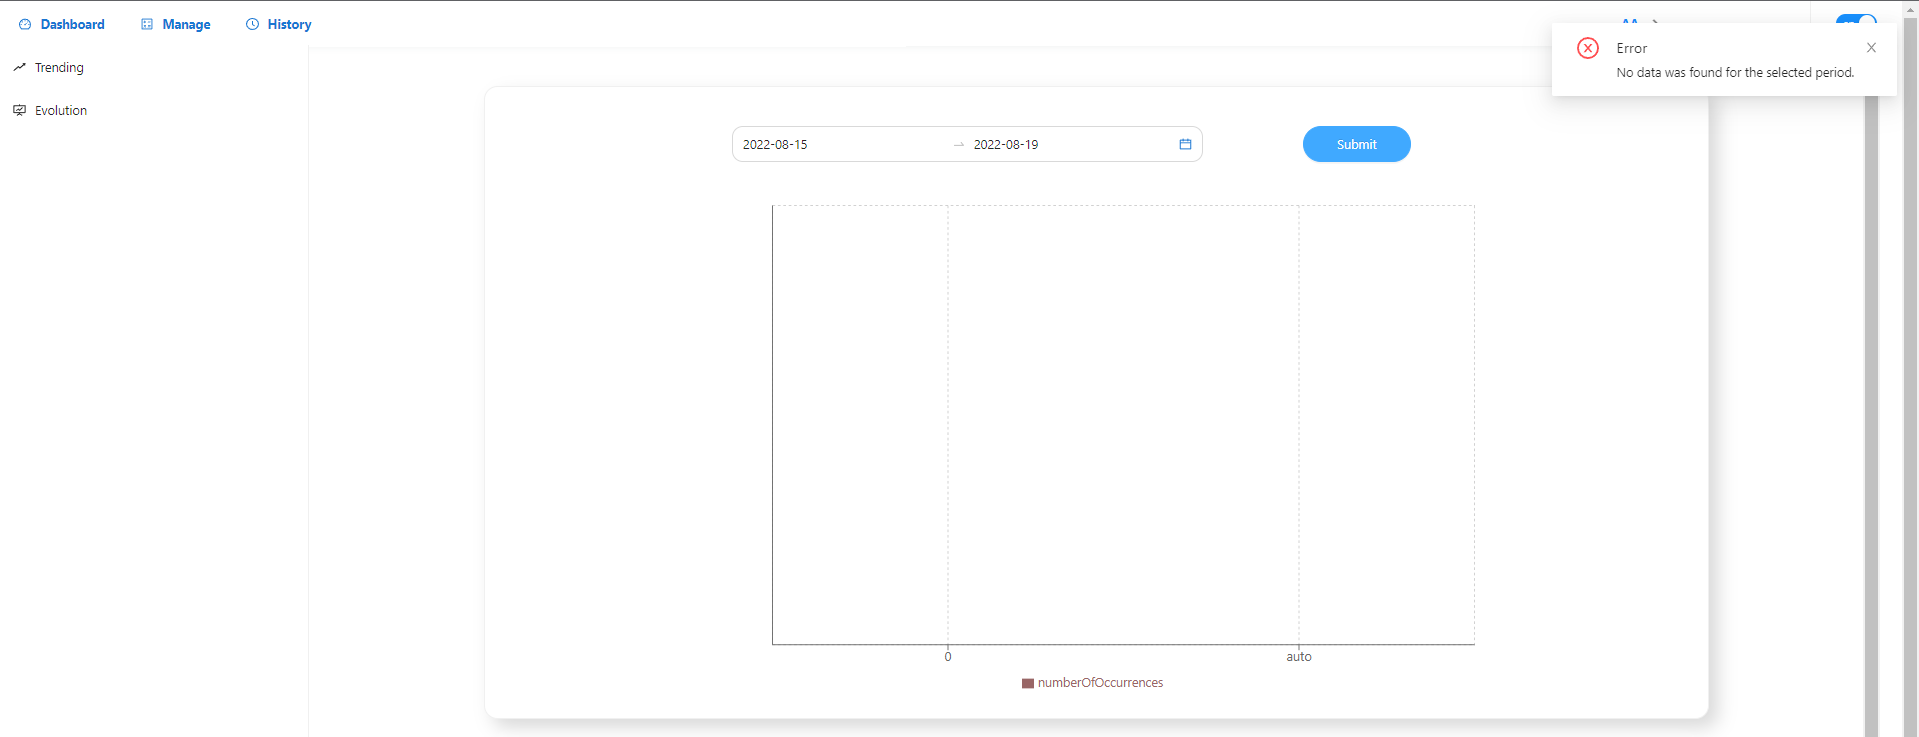
\includegraphics[width=150mm]{figs/trendingNoData.png}
    \caption{Grafic pentru top 10 cele mai populare subiecte - niciun rezultat}
	\label{fig:trendingNoData}
\end{figure}

\begin{figure}[h]
	\centering
	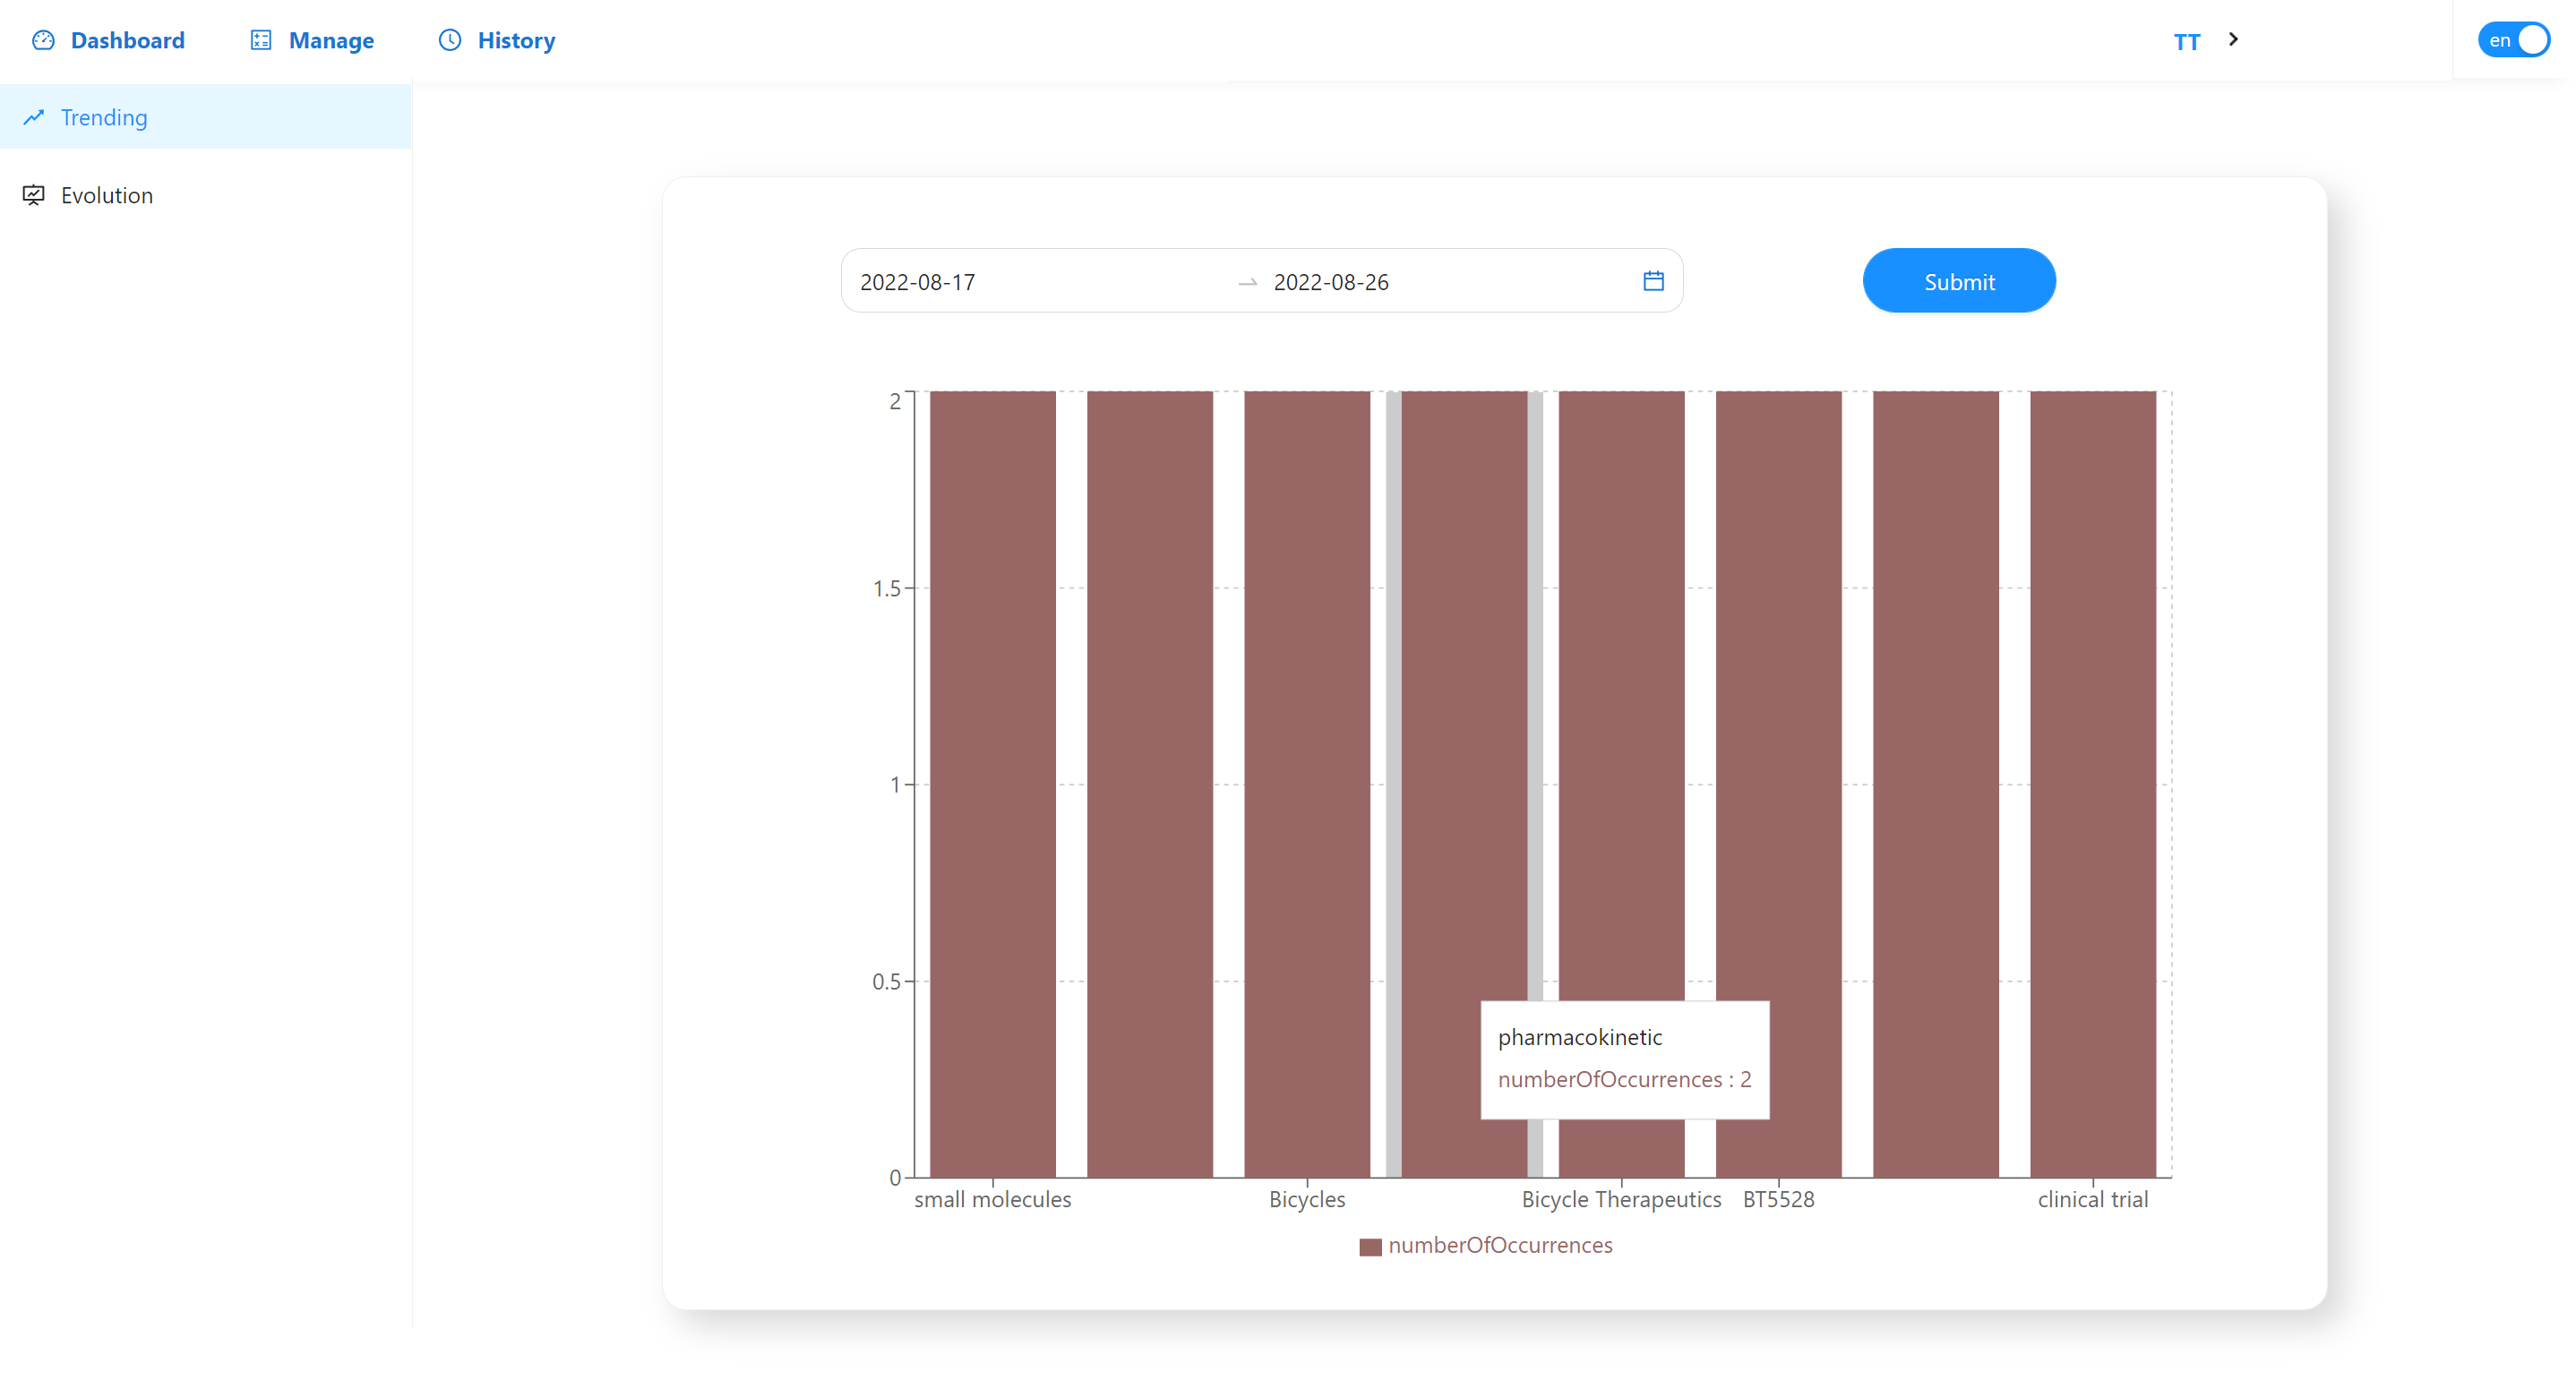
\includegraphics[width=150mm]{figs/trending.png}
    \caption{Grafic pentru top 10 cele mai populare subiecte}
	\label{fig:trending}
\end{figure}

\newpage
Alt element important pe care utilizatorul îl poate vedea aici este un WordCloud, care este, de fapt, o colecție de cuvinte sau expresii de diferite mărimi, ca în figura \ref{fig:wordcloud}. Mărimea este determinată de numărul total de apariții.
\begin{figure}[ht]
	\centering
	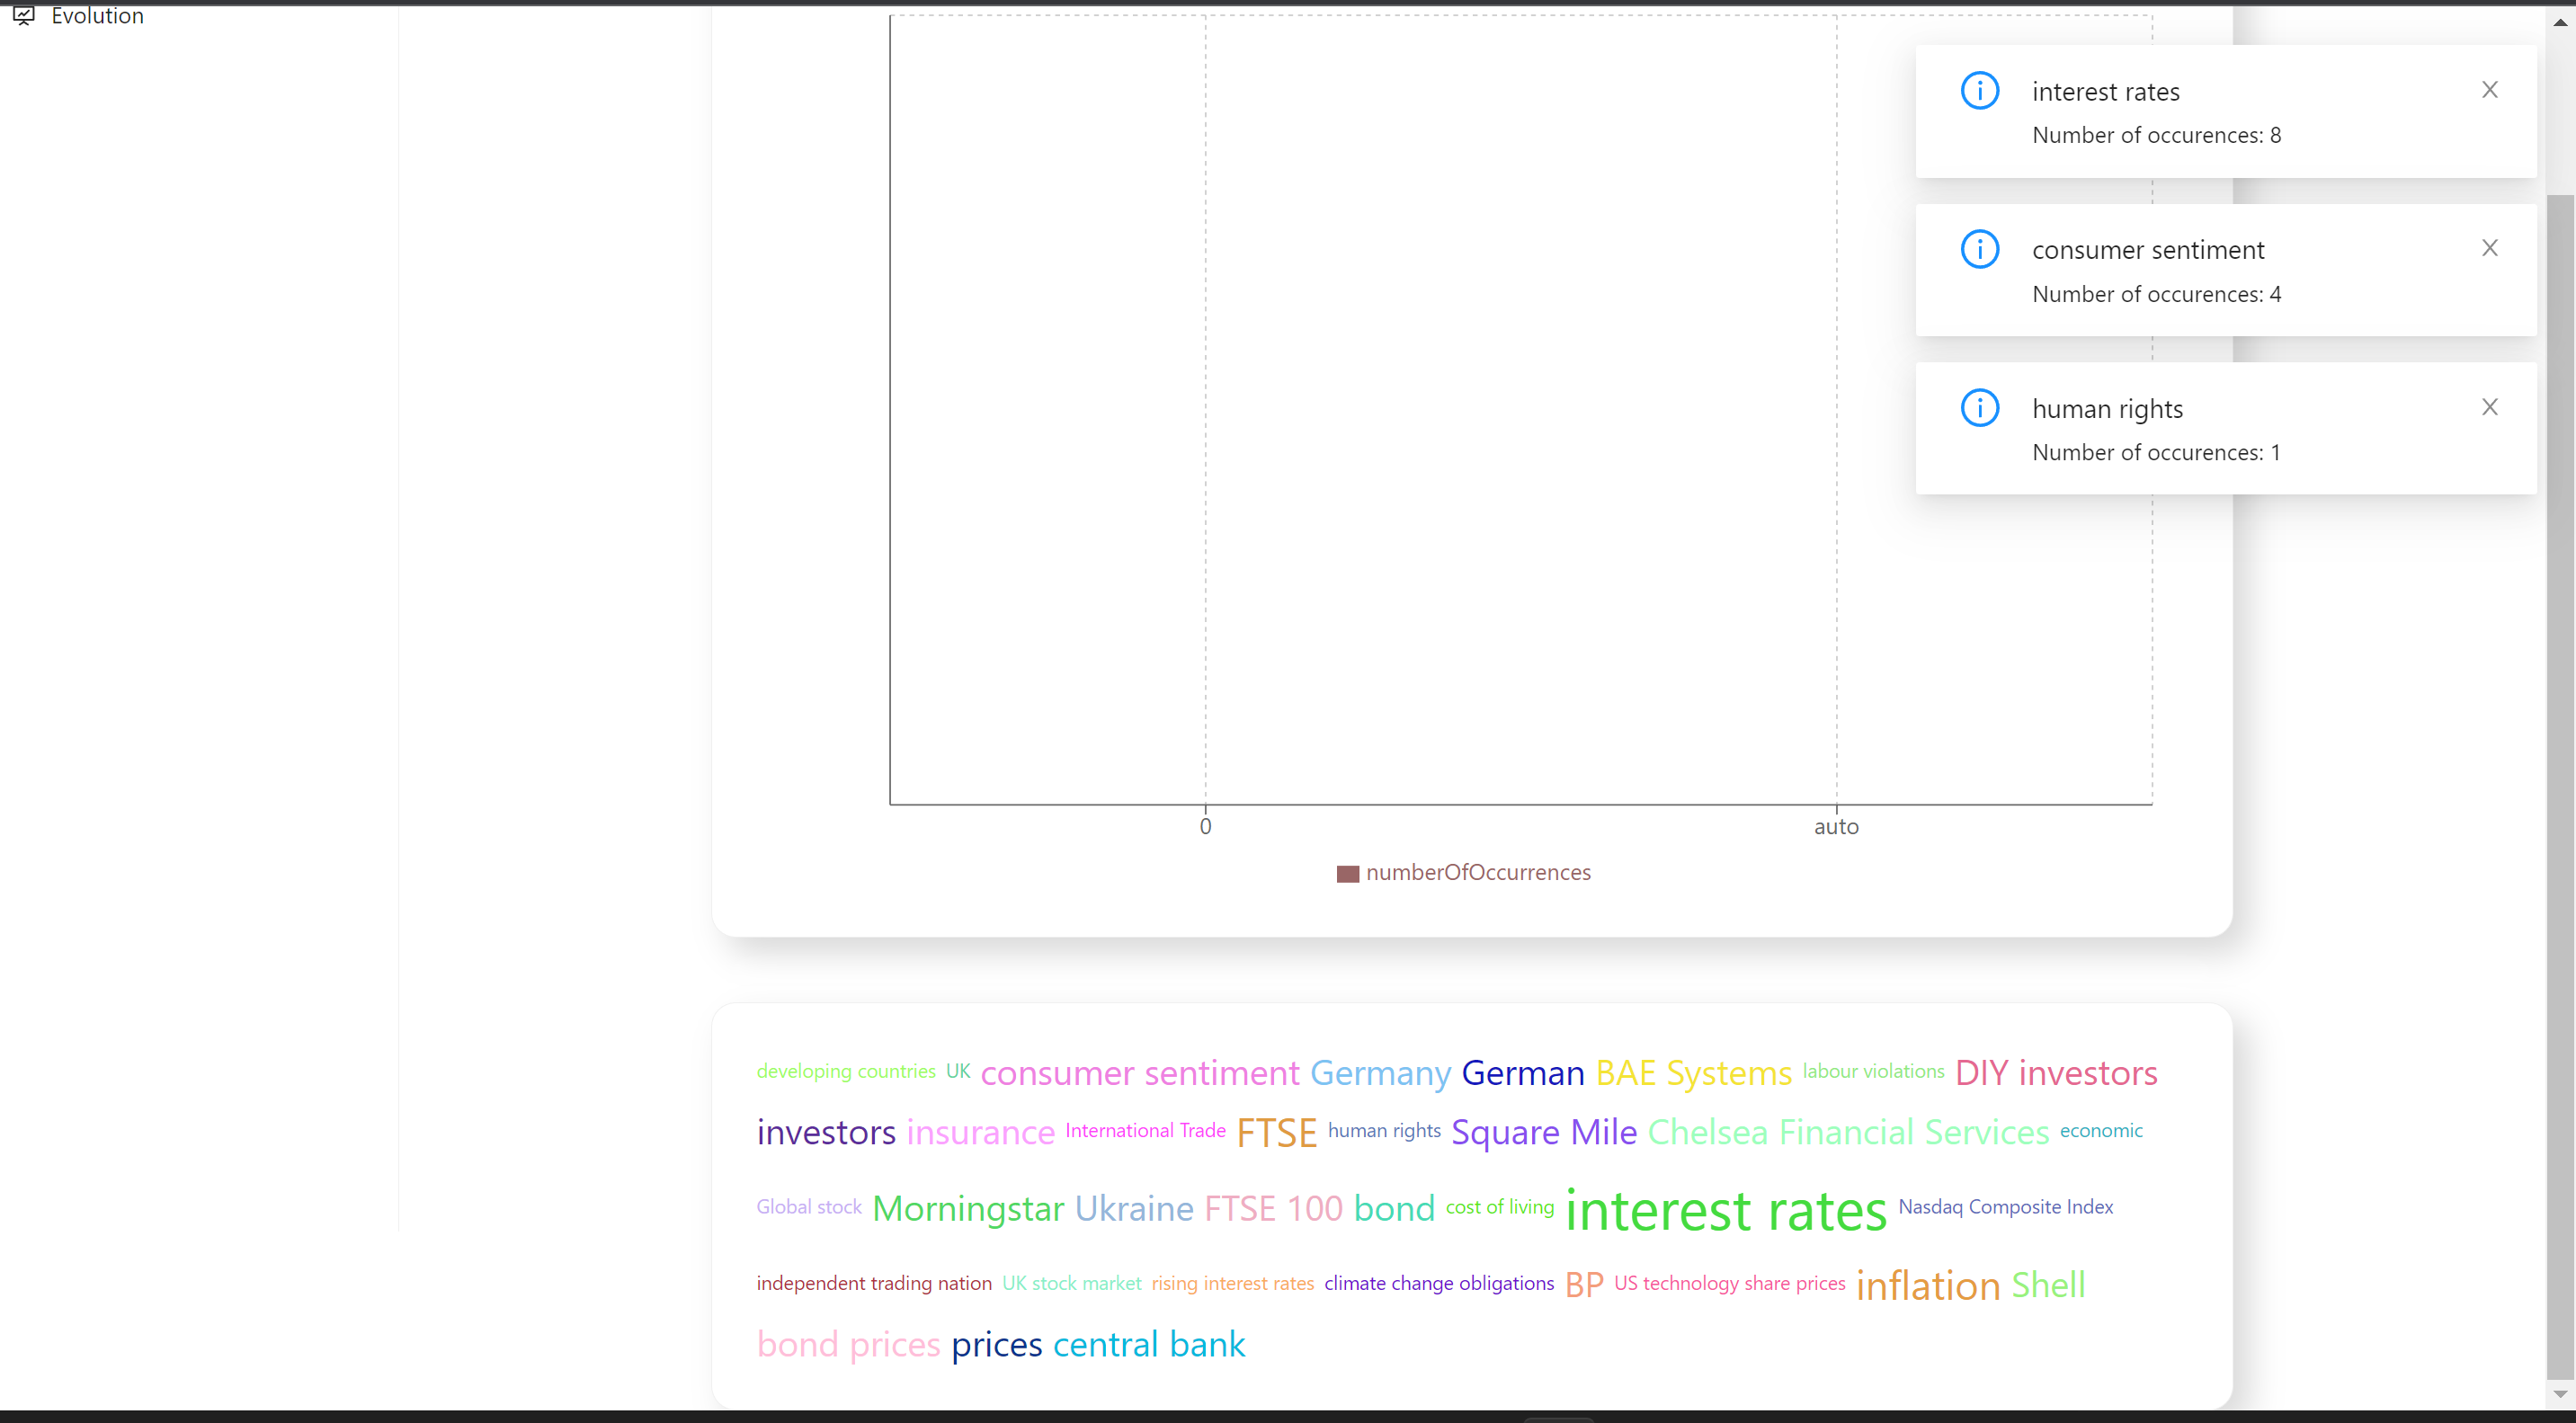
\includegraphics[width=150mm]{figs/wordcloud.png}
    \caption{WordCloud}
	\label{fig:wordcloud}
\end{figure}

\ \\
Evoluția unui cuvânt cheie sau expresie poate fi observată într-o perioadă de timp selectată.\\
La fel ca în cazul topicelor populare, dacă nu există date salvate pentru perioada sau inputul selectat, utilizatorul va fi notificat de acest lucru, ca în figura \ref{fig:evolutionNoData}. 
\begin{figure}[h]
	\centering
	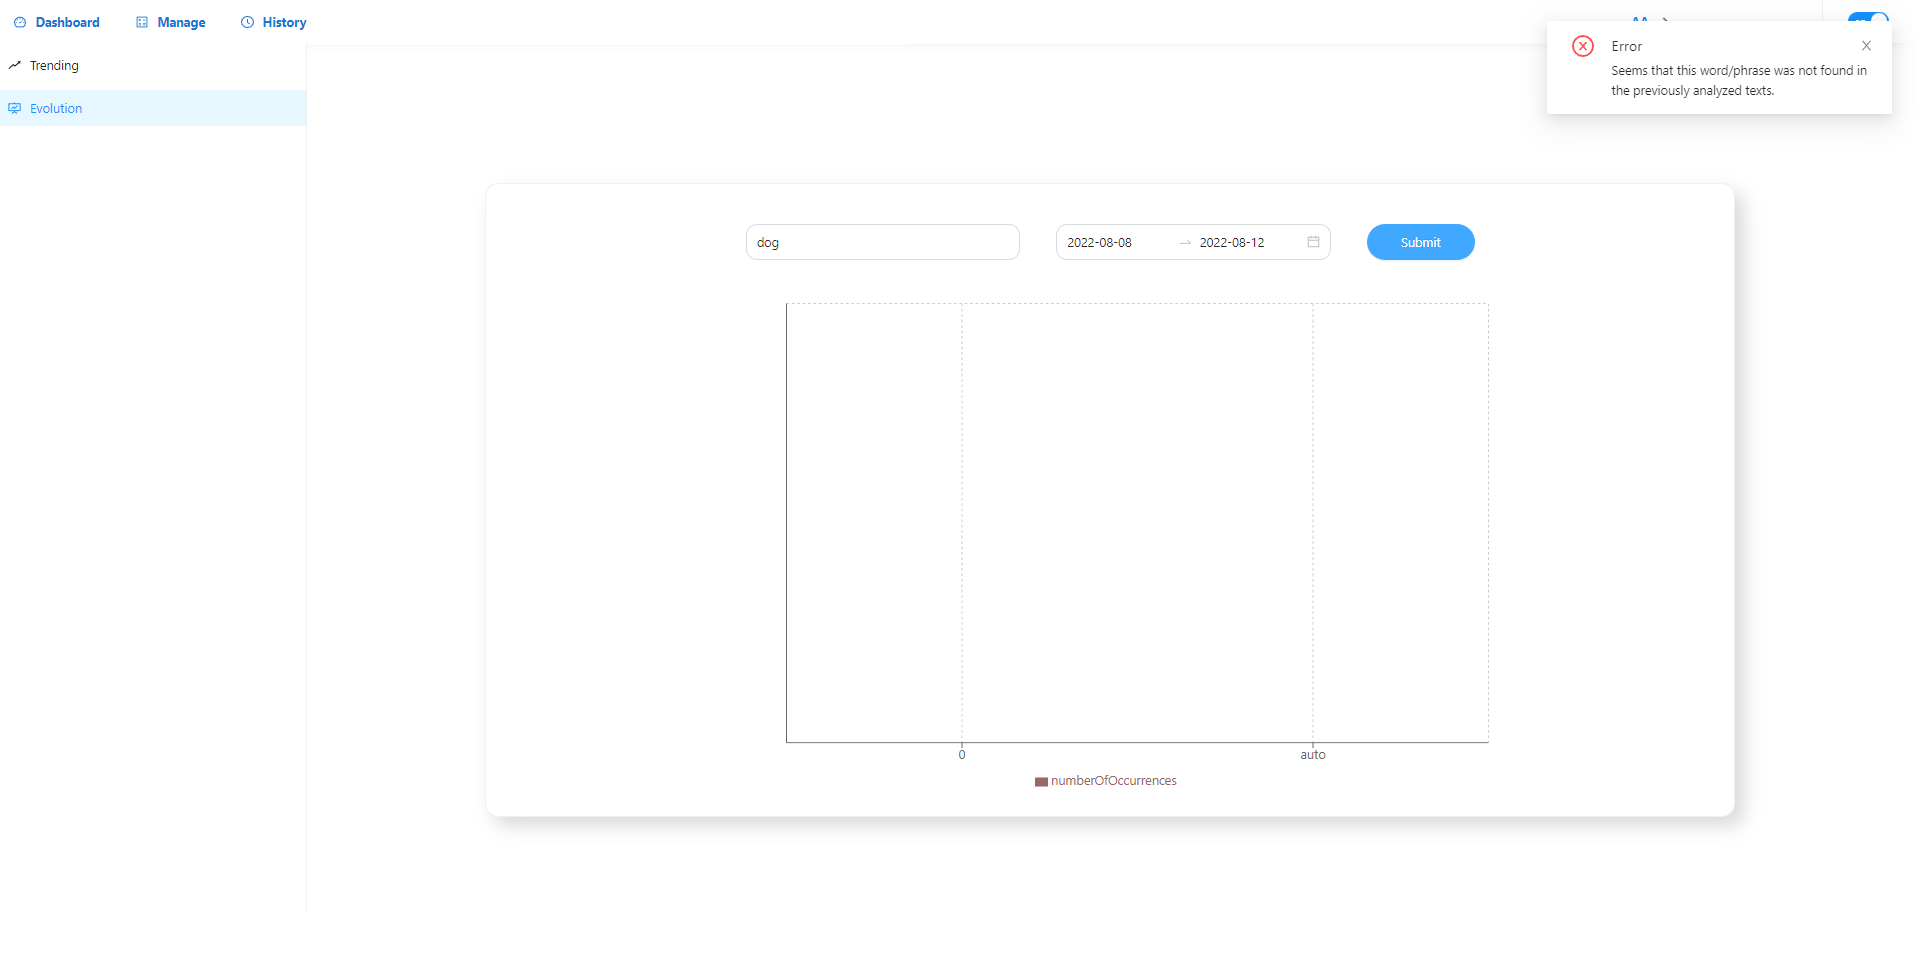
\includegraphics[width=150mm]{figs/evolutionNoData.png}
    \caption{Evoluția unui cuvânt cheie într-o anumită perioadă - niciun rezultat}
	\label{fig:evolutionNoData}
\end{figure}

\newpage
Altfel, în grafic se poate observa evoluția pe zile, ca în figura \ref{fig:evolution}.
\begin{figure}[t]
	\centering
	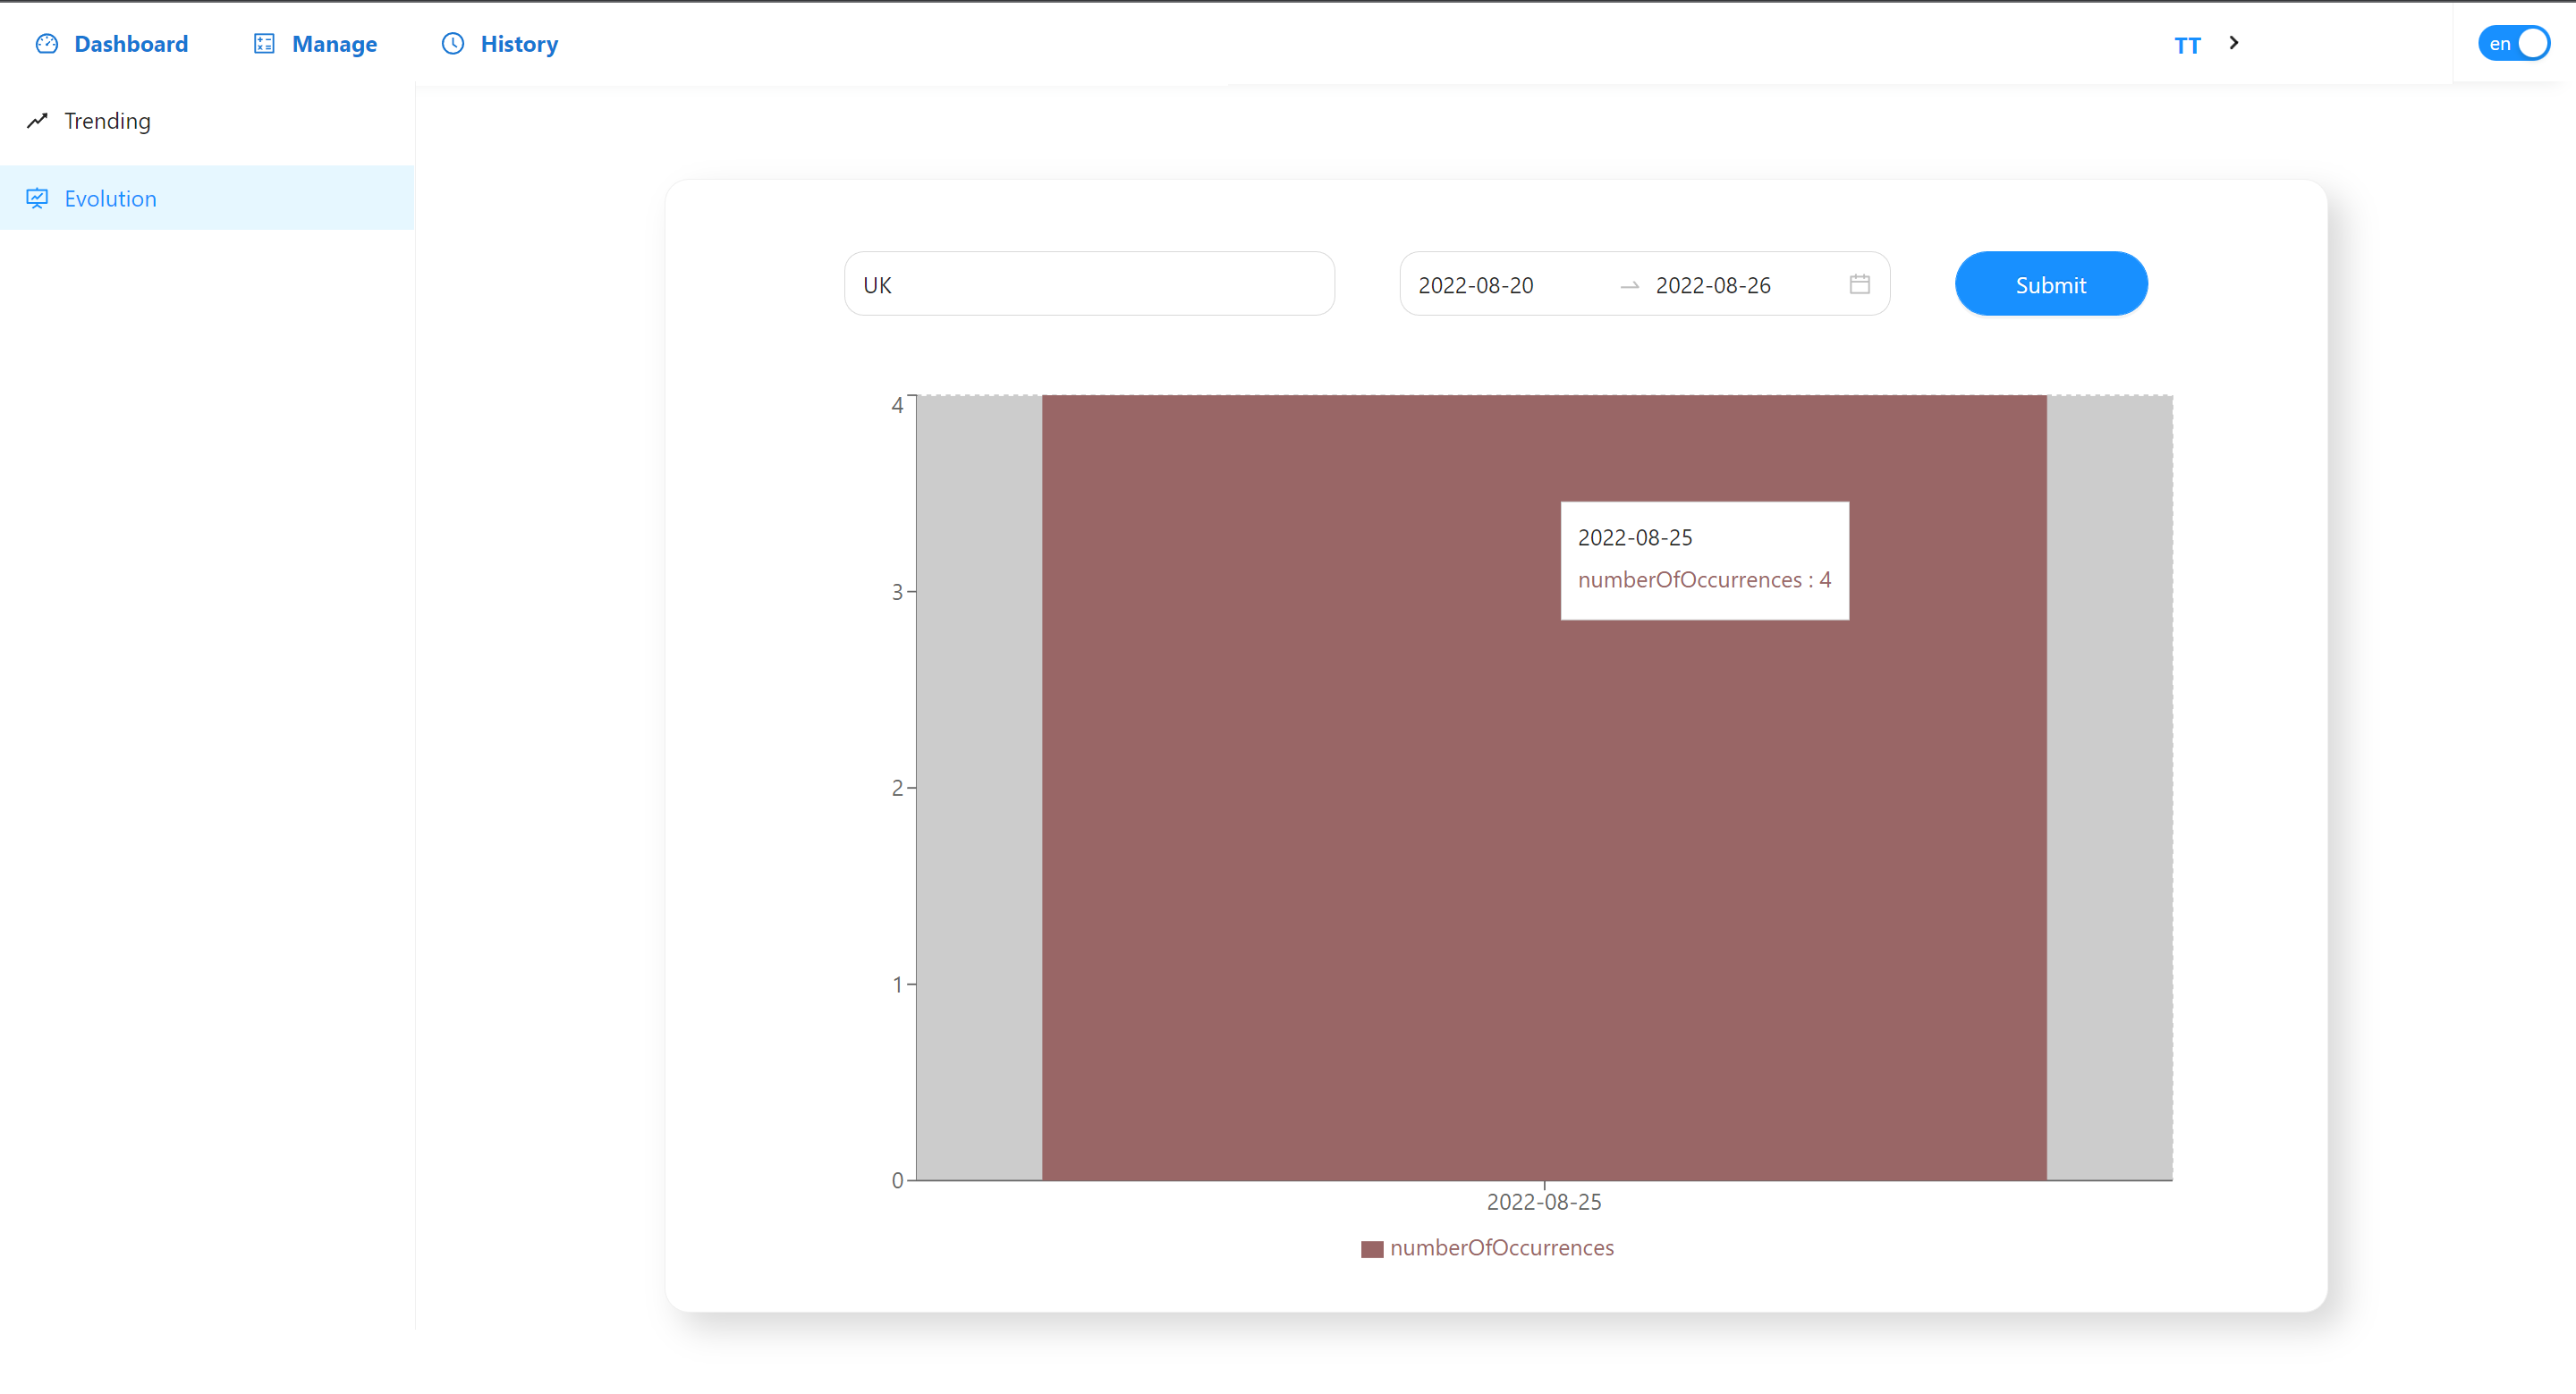
\includegraphics[width=150mm]{figs/evolution.png}
    \caption{Evoluția unui cuvânt cheie într-o anumită perioadă}
	\label{fig:evolution}
\end{figure}